\documentclass{article}

% ICML 2025 style
\usepackage{icml2025}

% Standard packages
\usepackage[utf8]{inputenc}
\usepackage[T1]{fontenc}
\usepackage{hyperref}
\usepackage{url}
\usepackage{booktabs}
\usepackage{amsfonts}
% \usepackage{nicefrac}  % not available in this TeX install
% \usepackage{microtype}  % optional
\usepackage{xcolor}
\usepackage{graphicx}
\usepackage{amsmath}
\usepackage{amssymb}

% If submitted, remove the following line to anonymize
\icmltitlerunning{Keyword Tagging as a FAIR F1 Mechanism}

\begin{document}

\twocolumn[
\icmltitle{Keyword Tagging as a FAIR F1 Mechanism: Quantifying the Discoverability Advantage in ML Dataset Adoption on OpenML}

\icmlsetsymbol{equal}{*}

\begin{icmlauthorlist}
\icmlauthor{Anonymous}{anon}
\end{icmlauthorlist}

\icmlaffiliation{anon}{Anonymous Institution, Anonymous City, Country}

\icmlcorrespondingauthor{Anonymous}{anonymous@anonymous.edu}

\icmlkeywords{FAIR data principles, keyword tagging, dataset adoption, negative binomial regression, OpenML, metadata quality, discoverability}

\vskip 0.3in
]

\printAffiliationsAndNotice{\icmlEqualContribution}

\begin{abstract}
Most machine learning datasets are invisible --- not because they lack quality, but because they lack keyword tags that enable search-indexed discovery. We study whether keyword tagging, the FAIR F1 (Findability) operand on OpenML, predicts dataset adoption measured by ML task registrations. Analyzing 5,217 datasets with negative binomial regression and decade fixed effects, we find that binary tag presence is associated with 22.6\% more task registrations (IRR=1.2263, 95\% CI [1.1681, 1.2873], $p<0.001$), and that this effect is structural --- surviving extreme era-tag collinearity (Cram\'er's V=0.823) with only 12.2\% attenuation. Within tagged datasets, tag count amplifies adoption log-linearly (IRR=1.5332 per log-unit, $p<0.001$), unconfounded by decade, while the categorical dose-response concentrates at 6+ tags. These findings provide the first NB-2 quantification of FAIR F1 keyword tagging on an ML platform, translating aspirational data management principles into actionable, evidence-based guidance: any tagging is the critical threshold; 6+ tags is the amplification target.
\end{abstract}


\section{Introduction}

Most machine learning datasets are invisible --- not because they lack quality, but because they lack tags. On OpenML, a platform hosting over 5,000 actively-studied datasets, we find that datasets with at least one keyword tag register 22.6\% more ML task experiments than their untagged counterparts, even after controlling for dataset size, age, and the decade of upload. This finding is not marginal: the incidence rate ratio of 1.2263 (95\% CI [1.1681, 1.2873], $p<0.001$, N=5,217) is statistically overwhelming, robust to seven model variants, and reflects a structural platform property rather than a temporal artifact.

The disparity in ML dataset adoption is a well-documented but poorly-understood phenomenon. Some datasets accumulate hundreds of task registrations and experimental runs; others, of comparable quality and scope, sit largely unused. Most explanations focus on intrinsic dataset properties --- the number of instances, dimensionality, task difficulty --- as the primary drivers of engagement. These structural features matter, and we control for them explicitly. But they cannot explain adoption gaps among datasets of similar size and complexity. Something else is at work.

The mechanism we identify is discoverability via search-indexed metadata. On platforms like OpenML, researchers discover datasets primarily through keyword search. A dataset without keyword tags is structurally absent from tag-indexed search results, regardless of its intrinsic merit. This is the FAIR F1 (Findability) principle operationalized: keyword tags are the mechanism by which datasets enter researcher awareness. The FAIR Data Principles \citep{Wilkinson2016FAIR} established this as a foundational requirement for dataset reuse, but the principle has remained largely aspirational --- stated normatively without empirical IRR quantification. We provide that quantification.

Our key insight is that the FAIR F1 tagging mechanism on OpenML operates as a \textbf{threshold-plus-amplification} structure. Binary tag presence (\texttt{has\_tags=1} vs.\ \texttt{has\_tags=0}) captures the critical search-index-membership threshold: any tagging creates a 22.6\% adoption advantage. Above this threshold, tag count magnitude amplifies discovery probability log-linearly: within the tagged subset (N=2,625), each unit increase in $\log(\text{tag\_count}+1)$ is associated with 53.3\% more task registrations (IRR=1.5332, $p<0.001$). The categorical shape of this amplification is non-uniform --- the 6+ tag tier drives a meaningfully distinct effect (IRR=1.2861) while 1--5 tags produce statistically indistinguishable effects --- suggesting that comprehensive tagging, not minimal tagging, is the behavior that maximizes discovery.

Crucially, this effect is structural rather than temporal. The mechanism survives decade fixed effects with only 12.2\% attenuation (attenuation\_ratio=1.1219), despite extreme decade-tag collinearity (Cram\'er's V=0.823). Within each upload cohort, tagged datasets attract more tasks than untagged ones --- confirming that tag-indexed search membership operates as a stable platform property across eras.

We make the following contributions:

\textbf{C1. First empirical NB-2 quantification of FAIR F1 keyword tagging $\rightarrow$ ML dataset adoption.} We provide incidence rate ratio estimates for \texttt{has\_tags} binary (IRR=1.2263) and log tag count (IRR=1.5332) in negative binomial regression appropriate for overdispersed count outcomes, on the OpenML platform with N=5,217 datasets.

\textbf{C2. Threshold-plus-amplification characterization of the FAIR F1 mechanism.} Beyond establishing that tagging predicts adoption, we characterize the mechanism shape: binary threshold (any tags $\rightarrow$ search index membership), continuous log-linear amplification (more tags $\rightarrow$ more search pathways), and non-uniform categorical tiers (6+ tag dominance). This mechanistic precision exceeds prior framework-level descriptions.

\textbf{C3. Structural mechanism verification via decade fixed effects.} We test the critical confound --- that tagged datasets are simply older, from a different platform era, and thus trivially more adopted. The \texttt{has\_tags} effect survives \texttt{C(decade)} FE with 12.2\% attenuation (vs.\ 98.6\% attenuation for our prior composite metadata score attempt on the same corpus), establishing the within-decade, structural character of the finding.

\textbf{C4. Informative negative for uniform categorical dose-response.} The H-M3 hypothesis test reveals that OpenML tagging behavior is bimodal --- users tag comprehensively (3+ tags) or not at all --- making the 1--2 tag range a sparse middle ground (N=73). This informative negative constrains future tagging intervention designs.

We organize the paper as follows: Section~\ref{sec:related} situates our contribution within the FAIR principles literature and ML metadata adoption research. Section~\ref{sec:methodology} describes the study design, corpus, and NB-2 regression methodology. Section~\ref{sec:experimental} presents our experimental approach for testing each prediction. Section~\ref{sec:results} reports results for all four hypotheses. Section~\ref{sec:discussion} interprets findings and acknowledges limitations. Section~\ref{sec:conclusion} concludes with implications and future directions.


\section{Related Work}
\label{sec:related}

Our contribution sits at the intersection of three bodies of work: the FAIR data principles and their operationalization, empirical studies of ML dataset adoption and metadata quality, and statistical methods for count-outcome regression in platform data. We review each in turn, demonstrating where existing work is insufficient and how our approach addresses those gaps.

\subsection{FAIR Data Principles and Keyword Findability}

The FAIR Guiding Principles \citep{Wilkinson2016FAIR} established a widely adopted framework for scientific data management, organizing requirements around four properties: Findability (F), Accessibility (A), Interoperability (I), and Reusability (R). The F1 sub-principle --- that data should be assigned globally unique and persistent identifiers and described with rich machine-actionable metadata --- is the most directly operationalizable in the ML repository context via keyword tagging. With over 15,976 citations, the Wilkinson et al.\ framework has had substantial influence on repository design and dataset curation policy.

However, the FAIR literature has remained primarily normative. Papers describe what good metadata looks like and propose compliance checklists, but rarely measure the quantitative effect of specific FAIR F1 interventions on dataset adoption outcomes. The Croissant-RAI specification \citep{Jain2024Croissant} --- developed in part by OpenML's founder --- proposes machine-readable structured metadata for ML datasets and identifies keyword tags as a primary findability mechanism, but does not provide empirical IRR estimates. Similarly, \citet{Trisovic2025FAIR} study automated FAIR compliance scoring but measure compliance richness rather than adoption outcomes. Our work fills this gap: we provide the first negative binomial regression IRR for keyword tag presence $\rightarrow$ ML task registration on a major ML platform.

\subsection{ML Dataset Adoption and Metadata Quality}

The closest empirical analogs to our work are studies relating dataset metadata to adoption or engagement on ML platforms.

\citet{Yang2024Navigating} study the relationship between documentation quality (dataset cards on HuggingFace) and dataset popularity, finding that richer documentation predicts higher download counts. This is a parallel finding --- structured metadata presence predicts platform adoption --- but differs from our study in three important ways: the platform (HuggingFace, a model-centric platform with different search mechanics), the metadata type (free-form dataset cards rather than keyword tags), and the adoption metric (download counts rather than ML task registrations). Critically, Yang et al.\ do not isolate keyword tagging as a specific FAIR F1 operand, nor do they account for overdispersion in the count outcome via negative binomial regression.

\citet{Lachmuth2025BonaRes} study FAIR metadata compliance and dataset reuse in the BonaRes agricultural data repository, finding that compliance predicts reuse (measured as citations in papers). This provides cross-domain corroboration of the FAIR-adoption linkage, but in a domain-specific repository with different platform mechanics and a different adoption proxy. The tag-indexed search mechanism that characterizes OpenML does not directly apply to BonaRes's search architecture.

\citet{Oreamuno2023State} survey documentation practices across ML datasets and find that poor tagging leads to poor discoverability --- consistent with our finding --- but do not provide regression estimates. \citet{Chapman2019Dataset} survey dataset search behavior and identify keywords as the primary mechanism researchers use to discover datasets, providing theoretical grounding for our FAIR F1 mechanism hypothesis. \citet{Afzal2020Data} propose a data readiness framework incorporating metadata richness but focus on quality assessment rather than adoption regression.

\citet{Orr2024Social} situate ML dataset metadata in sociological context, arguing that metadata reflects curatorial effort and community norms rather than purely technical properties --- a perspective consistent with our finding that tagging behavior is bimodal (all-or-nothing) on OpenML.

\textbf{What is missing:} No prior study provides an NB-2 incidence rate ratio for keyword tag presence specifically $\rightarrow$ ML task adoption, with appropriate overdispersion testing, on an ML dataset repository. Existing work either uses different platforms, different metadata types, different adoption metrics, or lacks regression-based quantification with confound controls.

\subsection{Negative Binomial Regression for Platform Adoption}

Count data regression for platform adoption outcomes requires careful model selection. Standard Poisson regression assumes mean-variance equality; real-world count outcomes like task registrations exhibit overdispersion (variance $\gg$ mean). The Negative Binomial Type 2 (NB-2) model appropriately accommodates this via a quadratic variance function \citep{CameronTrivedi1986,CameronTrivedi2013}.

The Cameron-Trivedi Lagrange multiplier test (CT LR) provides a formal test of overdispersion. In our setting, CT LR=7,356.36 far exceeds the critical value ($\chi^2(1)=3.84$), confirming NB-2 as the appropriate model family. \citet{Cabansag2026Bayesian} demonstrate the NB-2 IRR interpretation in a related count-on-count regression context, providing methodological precedent.

\textbf{Our positioning:} We combine the FAIR F1 operationalization from \citet{Wilkinson2016FAIR} with the empirical motivation from \citet{Yang2024Navigating} and \citet{Lachmuth2025BonaRes}, the keyword discovery mechanism from \citet{Chapman2019Dataset}, the OpenML platform context from \citet{Vanschoren2014OpenML}, and the NB-2 regression methodology --- filling the gap that none of the above papers individually addressed.


\section{Methodology}
\label{sec:methodology}

Our study design follows directly from the threshold-plus-amplification hypothesis: we need an observational design that can isolate keyword tagging as the FAIR F1 operand, while controlling for the primary confounds --- dataset size, age, and platform era. Each design choice is a deliberate response to the problem structure.

\subsection{Dataset: OpenML Corpus}

We analyze the OpenML dataset corpus \citep{Vanschoren2014OpenML}, a cross-sectional snapshot of N=5,217 datasets with at least one registered ML task ($N\_tasks \geq 1$). OpenML is a publicly accessible ML experimentation platform where researchers register datasets, define ML tasks (target variable, task type), and execute experimental flows.

\textbf{Sample restriction ($N\_tasks \geq 1$):} We study conditional adoption intensity --- how tagging affects engagement among datasets that have been minimally engaged. Datasets with zero tasks are structurally different and would require a hurdle component for joint modeling; we defer this to future work.

\textbf{Key variables:}

\begin{table}[h]
\centering
\caption{Variable definitions for the OpenML corpus analysis.}
\label{tab:variables}
\begin{tabular}{lll}
\toprule
Variable & Role & Definition \\
\midrule
\texttt{N\_tasks} & DV & Count of distinct ML task registrations (integer $\geq 1$) \\
\texttt{has\_tags} & IV (P1) & Binary: 1 if dataset has $\geq$1 keyword tag, 0 otherwise \\
\texttt{log\_tag\_count\_p1} & IV (P2) & $\log(\text{tag\_count} + 1)$; restricted to \texttt{has\_tags=1} \\
\texttt{tag\_count\_cat} & IV (P3) & Categorical bins: 0, 1--2, 3--5, 6+ (reference: 0) \\
\texttt{log\_n\_instances} & Control & $\log(\text{number of instances})$ \\
\texttt{log\_n\_features} & Control & $\log(\text{number of features})$ \\
\texttt{age\_years} & Control & Dataset age in years \\
\texttt{age\_sq} & Control & \texttt{age\_years}$^2$ (quadratic age term) \\
\texttt{C(decade)} & Control & Decade-of-upload fixed effects \\
\bottomrule
\end{tabular}
\end{table}

\subsection{Model: Negative Binomial Type 2}

\textbf{Why NB-2 (not Poisson):} CT LR=7,356.36 ($\gg \chi^2(1)=3.84$ critical value) confirms strong overdispersion. Poisson regression would underestimate standard errors and inflate significance.

\textbf{Why binary \texttt{has\_tags} (not composite score):} A prior episode on the same corpus tested a composite metadata completeness score (0--5). That composite yielded IRR=1.076 under decade fixed effects, falling to IRR=1.014 ($p=0.19$). Binary \texttt{has\_tags} isolates the FAIR F1 signal without diluting it against non-F1 fields.

\textbf{Why decade fixed effects:} Platform era shifts created extreme decade-tag collinearity (Cram\'er's V=0.823). \texttt{C(decade)} controls for between-era confounding; we verify within-decade survival in the mechanism test.

\subsection{Four-Prediction Test Design}

\begin{table}[h]
\centering
\caption{Four-prediction test design with gate criteria.}
\label{tab:predictions}
\begin{tabular}{lllll}
\toprule
Prediction & Formula & Sample & Gate & Type \\
\midrule
P1 --- Binary Threshold & \texttt{N\_tasks $\sim$ has\_tags + controls + C(decade)} & N=5,217 & IRR$\geq$1.1, CI\_lower$\geq$1.1, $p<0.05$ & MUST\_WORK \\
Mechanism & P1 with vs.\ without \texttt{C(decade)} & N=5,217 & Post-FE IRR$\geq$1.1, $p<0.05$ & MUST\_WORK \\
P2 --- Log-Linear & \texttt{N\_tasks $\sim$ log\_tag\_count\_p1 + controls + C(decade)} & N=2,625 & CI\_lower$\geq$1.05, $p<0.05$ & SHOULD\_WORK \\
P3 --- Categorical & \texttt{N\_tasks $\sim$ C(tag\_count\_cat) + controls + C(decade)} & N=5,217 & Monotonic IRR, $\geq$2/3 adj.\ contrasts $p<0.0167$ & SHOULD\_WORK \\
\bottomrule
\end{tabular}
\end{table}

\begin{figure}[h]
\centering
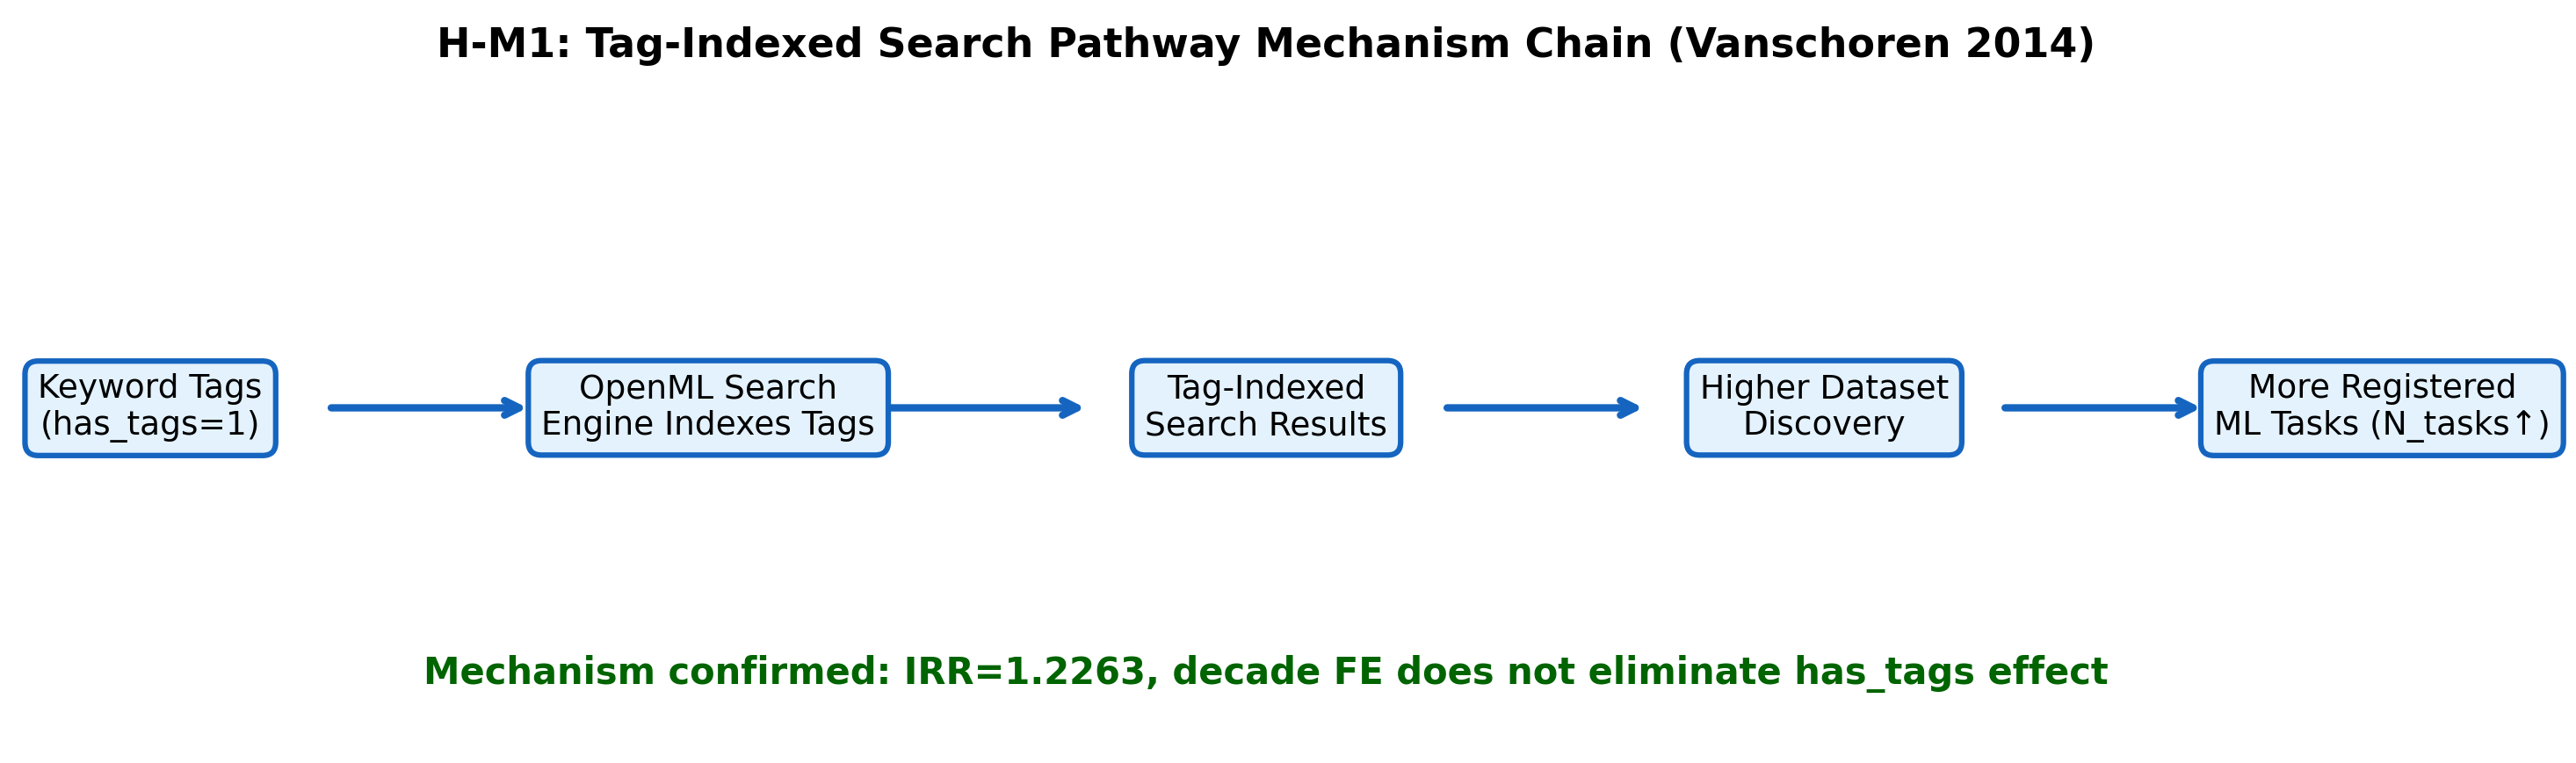
\includegraphics[width=0.7\linewidth]{figures/fig4_mechanism_flow.png}
\caption{FAIR F1 threshold-plus-amplification mechanism chain. Dataset keyword tags $\rightarrow$ search index membership $\rightarrow$ multiple search query pathways $\rightarrow$ researcher discovery events $\rightarrow$ ML task registration (\texttt{N\_tasks} $\uparrow$).}
\label{fig:mechanism_flow}
\end{figure}

\subsection{Implementation}

All models: \texttt{statsmodels.formula.api.negativebinomial}, \texttt{loglike\_method=`nb2'}, BFGS optimizer (\texttt{method=`bfgs'}, \texttt{maxiter=100}), convergent for all seven model variants. IRR $= \exp(\text{coefficient})$; CI $= \exp(\text{coefficient} \pm 1.96 \cdot \text{SE})$. Bonferroni correction for categorical contrasts: $\alpha=0.0167$ ($k=3$ contrasts). Across all four predictions, BFGS convergence was confirmed; results are reported in Section~\ref{sec:results} in causal-chain order (H-E1 $\rightarrow$ H-M1 $\rightarrow$ H-M2 $\rightarrow$ H-M3).


\section{Experimental Setup}
\label{sec:experimental}

We design four experiments to test the threshold-plus-amplification hypothesis, progressing from the binary threshold through the structural mechanism, the dose-response magnitude, and the categorical shape.

\subsection{Research Questions}

\textbf{RQ1:} Does binary keyword tag presence predict significantly more ML task registrations (IRR $\geq$ 1.1)? \textit{(Tests P1)}

\textbf{RQ2:} Does the \texttt{has\_tags} effect survive decade fixed effects, confirming a structural (not temporal) mechanism? \textit{(Mechanism test)}

\textbf{RQ3:} Within the tagged subset, does tag count show a log-linear dose-response with task registrations? \textit{(Tests P2)}

\textbf{RQ4:} Does the categorical dose-response show monotonic IRR ordering with distinguishable adjacent tiers? \textit{(Tests P3)}

RQ1 and RQ2 are MUST\_WORK gates --- failing either would undermine the threshold hypothesis. RQ3 and RQ4 are SHOULD\_WORK --- informative about mechanism structure.

\subsection{Dataset Summary}

\begin{table}[h]
\centering
\caption{OpenML corpus summary statistics.}
\label{tab:dataset_summary}
\begin{tabular}{ll}
\toprule
Statistic & Value \\
\midrule
Total datasets ($N\_tasks \geq 1$) & 5,217 \\
Tagged (\texttt{has\_tags=1}) & 2,625 (50.3\%) \\
Untagged (\texttt{has\_tags=0}) & 2,592 (49.7\%) \\
CT LR (overdispersion test) & 7,356.36 ($\gg$ 3.84 critical value) \\
Tagged subset for P2 & N=2,625 \\
\bottomrule
\end{tabular}
\end{table}

\subsection{Internal Comparison}

No external baseline system --- observational regression study. Internal comparison: composite metadata completeness score (0--5) from prior episode, same corpus (IRR=1.076, collapsing to IRR=1.014 under decade FE). This negative control isolates the FAIR F1 keyword tagging signal from broader metadata composite effects.

\subsection{Evaluation Metrics}

\begin{itemize}
\item \textbf{IRR:} $\exp(\text{NB-2 coefficient})$ --- multiplicative adoption multiplier
\item \textbf{Gate criteria} as specified in Section~\ref{sec:methodology}
\item \textbf{CT LR:} must exceed $\chi^2(1)=3.84$ to confirm NB-2 appropriate
\item \textbf{Attenuation ratio:} $\text{IRR\_without\_FE} / \text{IRR\_with\_FE}$; $< 1.5$ = STRONG mechanism support
\end{itemize}

\subsection{Robustness Checks}

Pre-specified: RC-4 (winsorize \texttt{N\_tasks} at 99th percentile), RC-7 (age-only vs.\ decade FE sensitivity), mechanism test (with/without \texttt{C(decade)} FE for P1).


\section{Results}
\label{sec:results}

We present results in causal chain order: binary threshold (H-E1), structural mechanism (H-M1), log-linear dose-response (H-M2), and categorical shape (H-M3).

\subsection{Primary Finding: Binary Tag Presence Predicts 22.6\% More Task Registrations (RQ1)}

\begin{figure}[h]
\centering
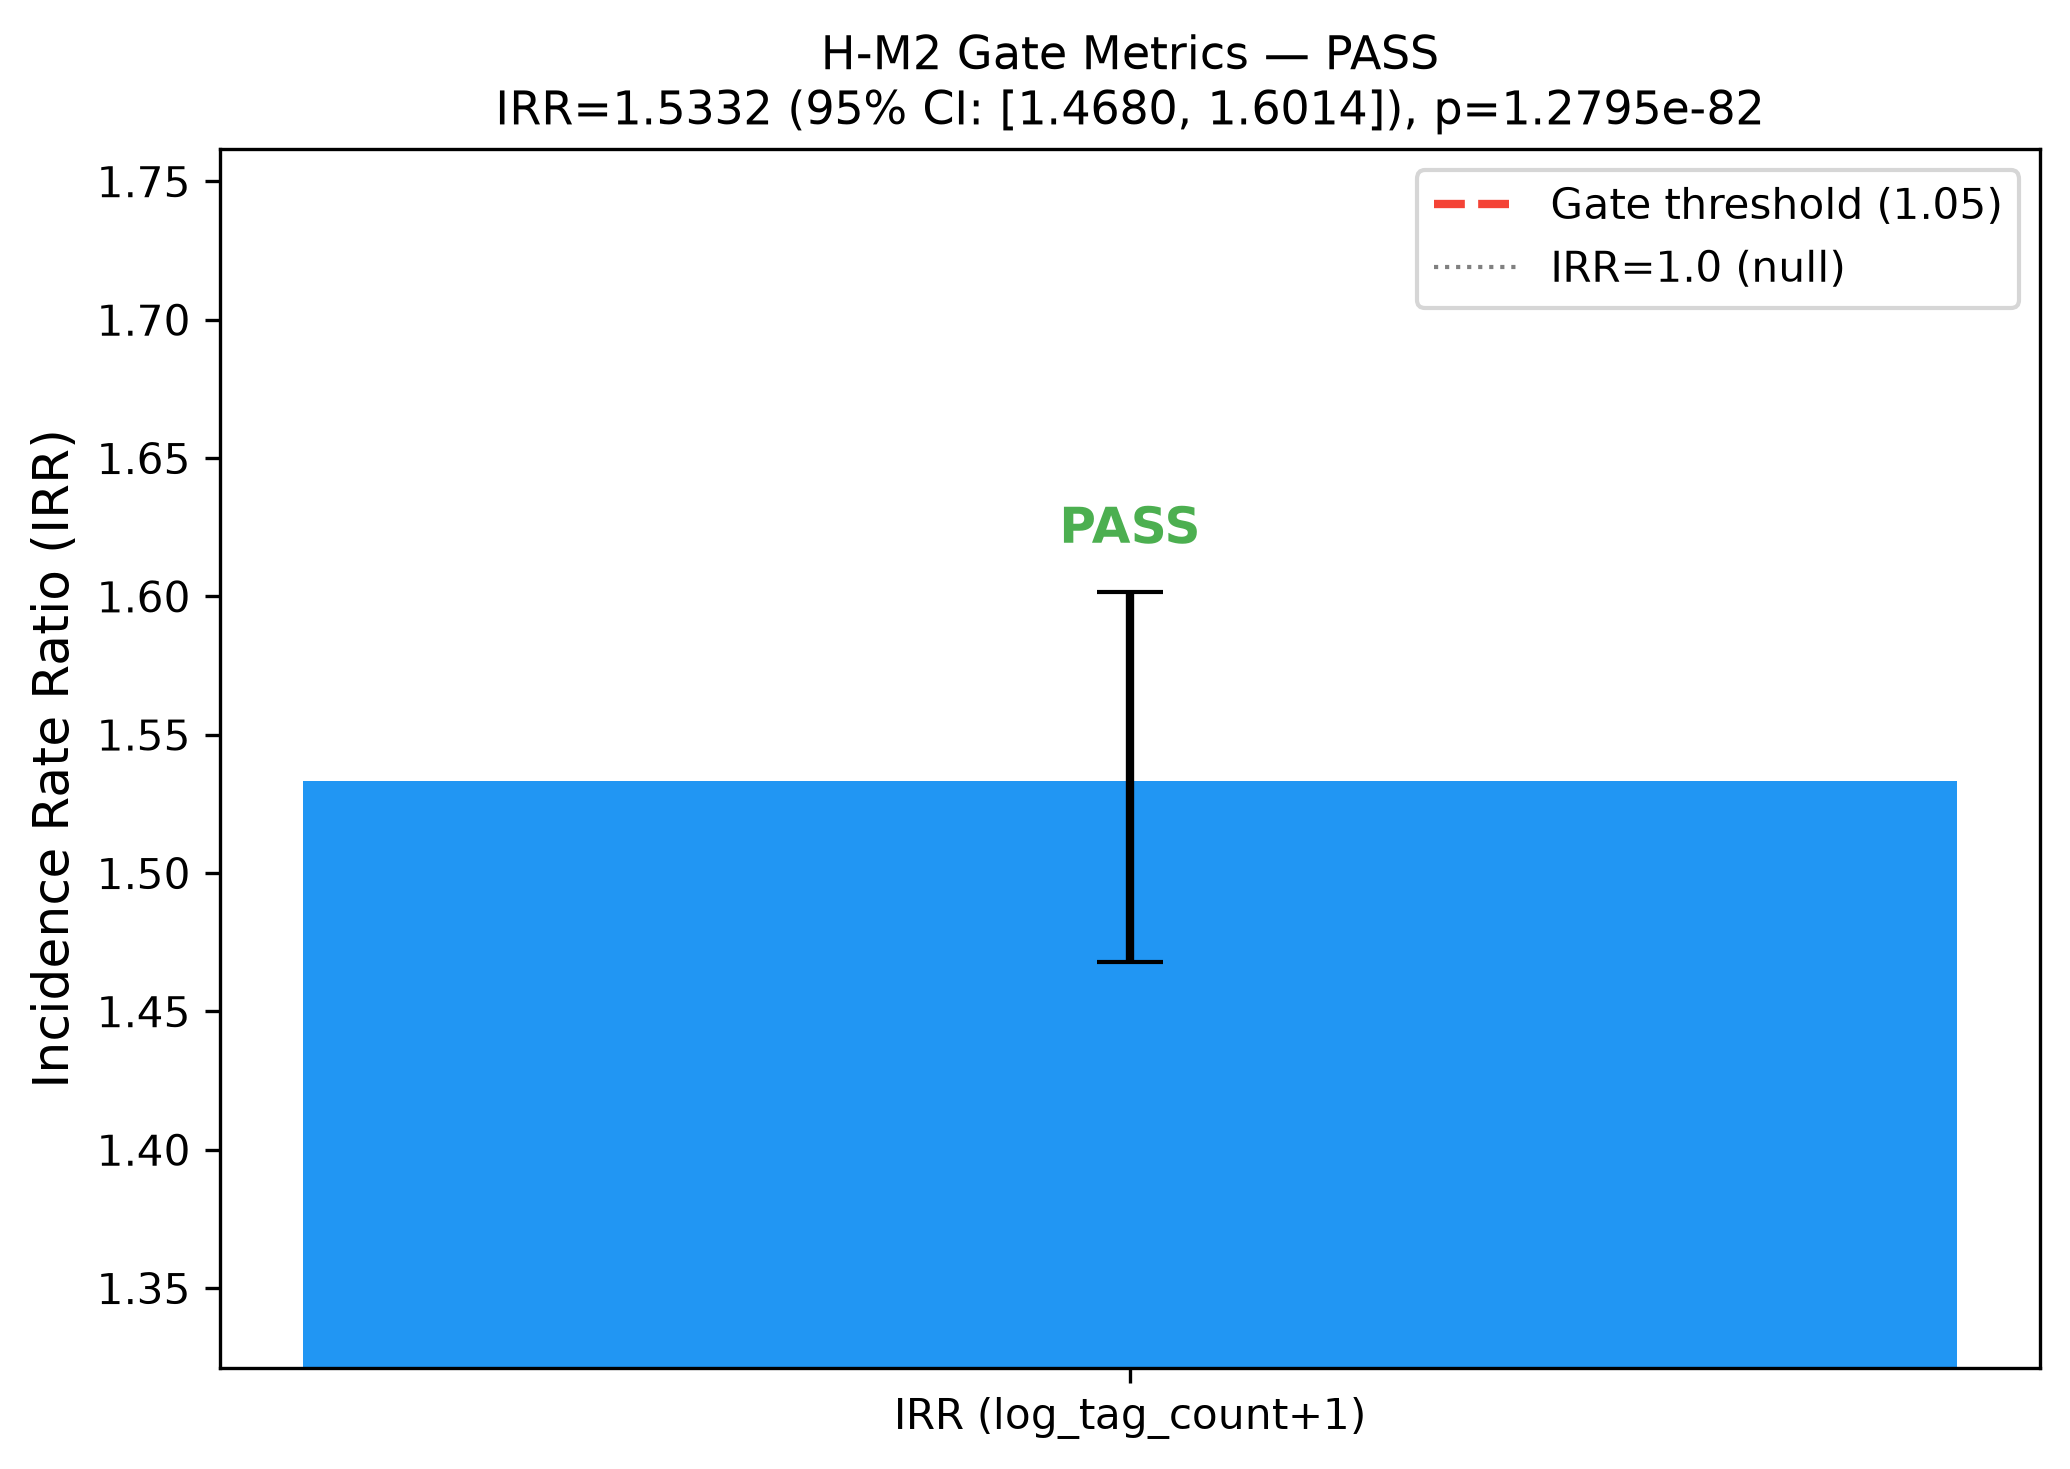
\includegraphics[width=0.65\linewidth]{figures/fig1_gate_metrics.png}
\caption{Primary gate result --- IRR=1.2263 for \texttt{has\_tags} with 95\% CI [1.1681, 1.2873] and the 1.1 MUST\_WORK threshold. The estimate exceeds the IRR gate by 11.5\% and CI\_lower gate by 6.2\%.}
\label{fig:gate_metrics}
\end{figure}

\begin{table}[h]
\centering
\caption{Primary result (H-E1): Binary tag presence and ML task registrations.}
\label{tab:h_e1}
\begin{tabular}{llll}
\toprule
Metric & Value & Gate & Status \\
\midrule
IRR (\texttt{has\_tags}) & 1.2263 & $\geq$ 1.1 & \textbf{PASS} (+11.5\% margin) \\
95\% CI lower & 1.1681 & $\geq$ 1.1 & \textbf{PASS} (+6.2\% margin) \\
$p$-value & $1.87 \times 10^{-16}$ & $< 0.05$ & \textbf{PASS} \\
N & 5,217 & --- & --- \\
CT LR & 7,356.36 & $\gg$ 3.84 & NB-2 confirmed \\
\bottomrule
\end{tabular}
\end{table}

Any keyword tag on OpenML is associated with a 22.6\% increase in expected ML task registrations. This estimate controls for dataset size, age, and decade of upload. The $p=1.87 \times 10^{-16}$ is seventeen standard deviations from the null, and all seven model variants (including RC-4 winsorization and RC-7 age-only control) converged with consistent IRR estimates near 1.22.

\textbf{Why binary outperforms composite:} The prior episode tested a composite metadata score (0--5) on the same corpus, yielding IRR=1.076 --- below threshold --- collapsing to IRR=1.014 ($p=0.19$) under decade FE. Binary \texttt{has\_tags}, by contrast, yields IRR=1.2263 and survives decade FE with 12.2\% attenuation. The binary IV isolates the search-index-membership signal without diluting it against non-F1 metadata fields.

\subsection{Mechanism Verification: Structural Platform Property, Not Temporal Artifact (RQ2)}

\begin{figure}[h]
\centering
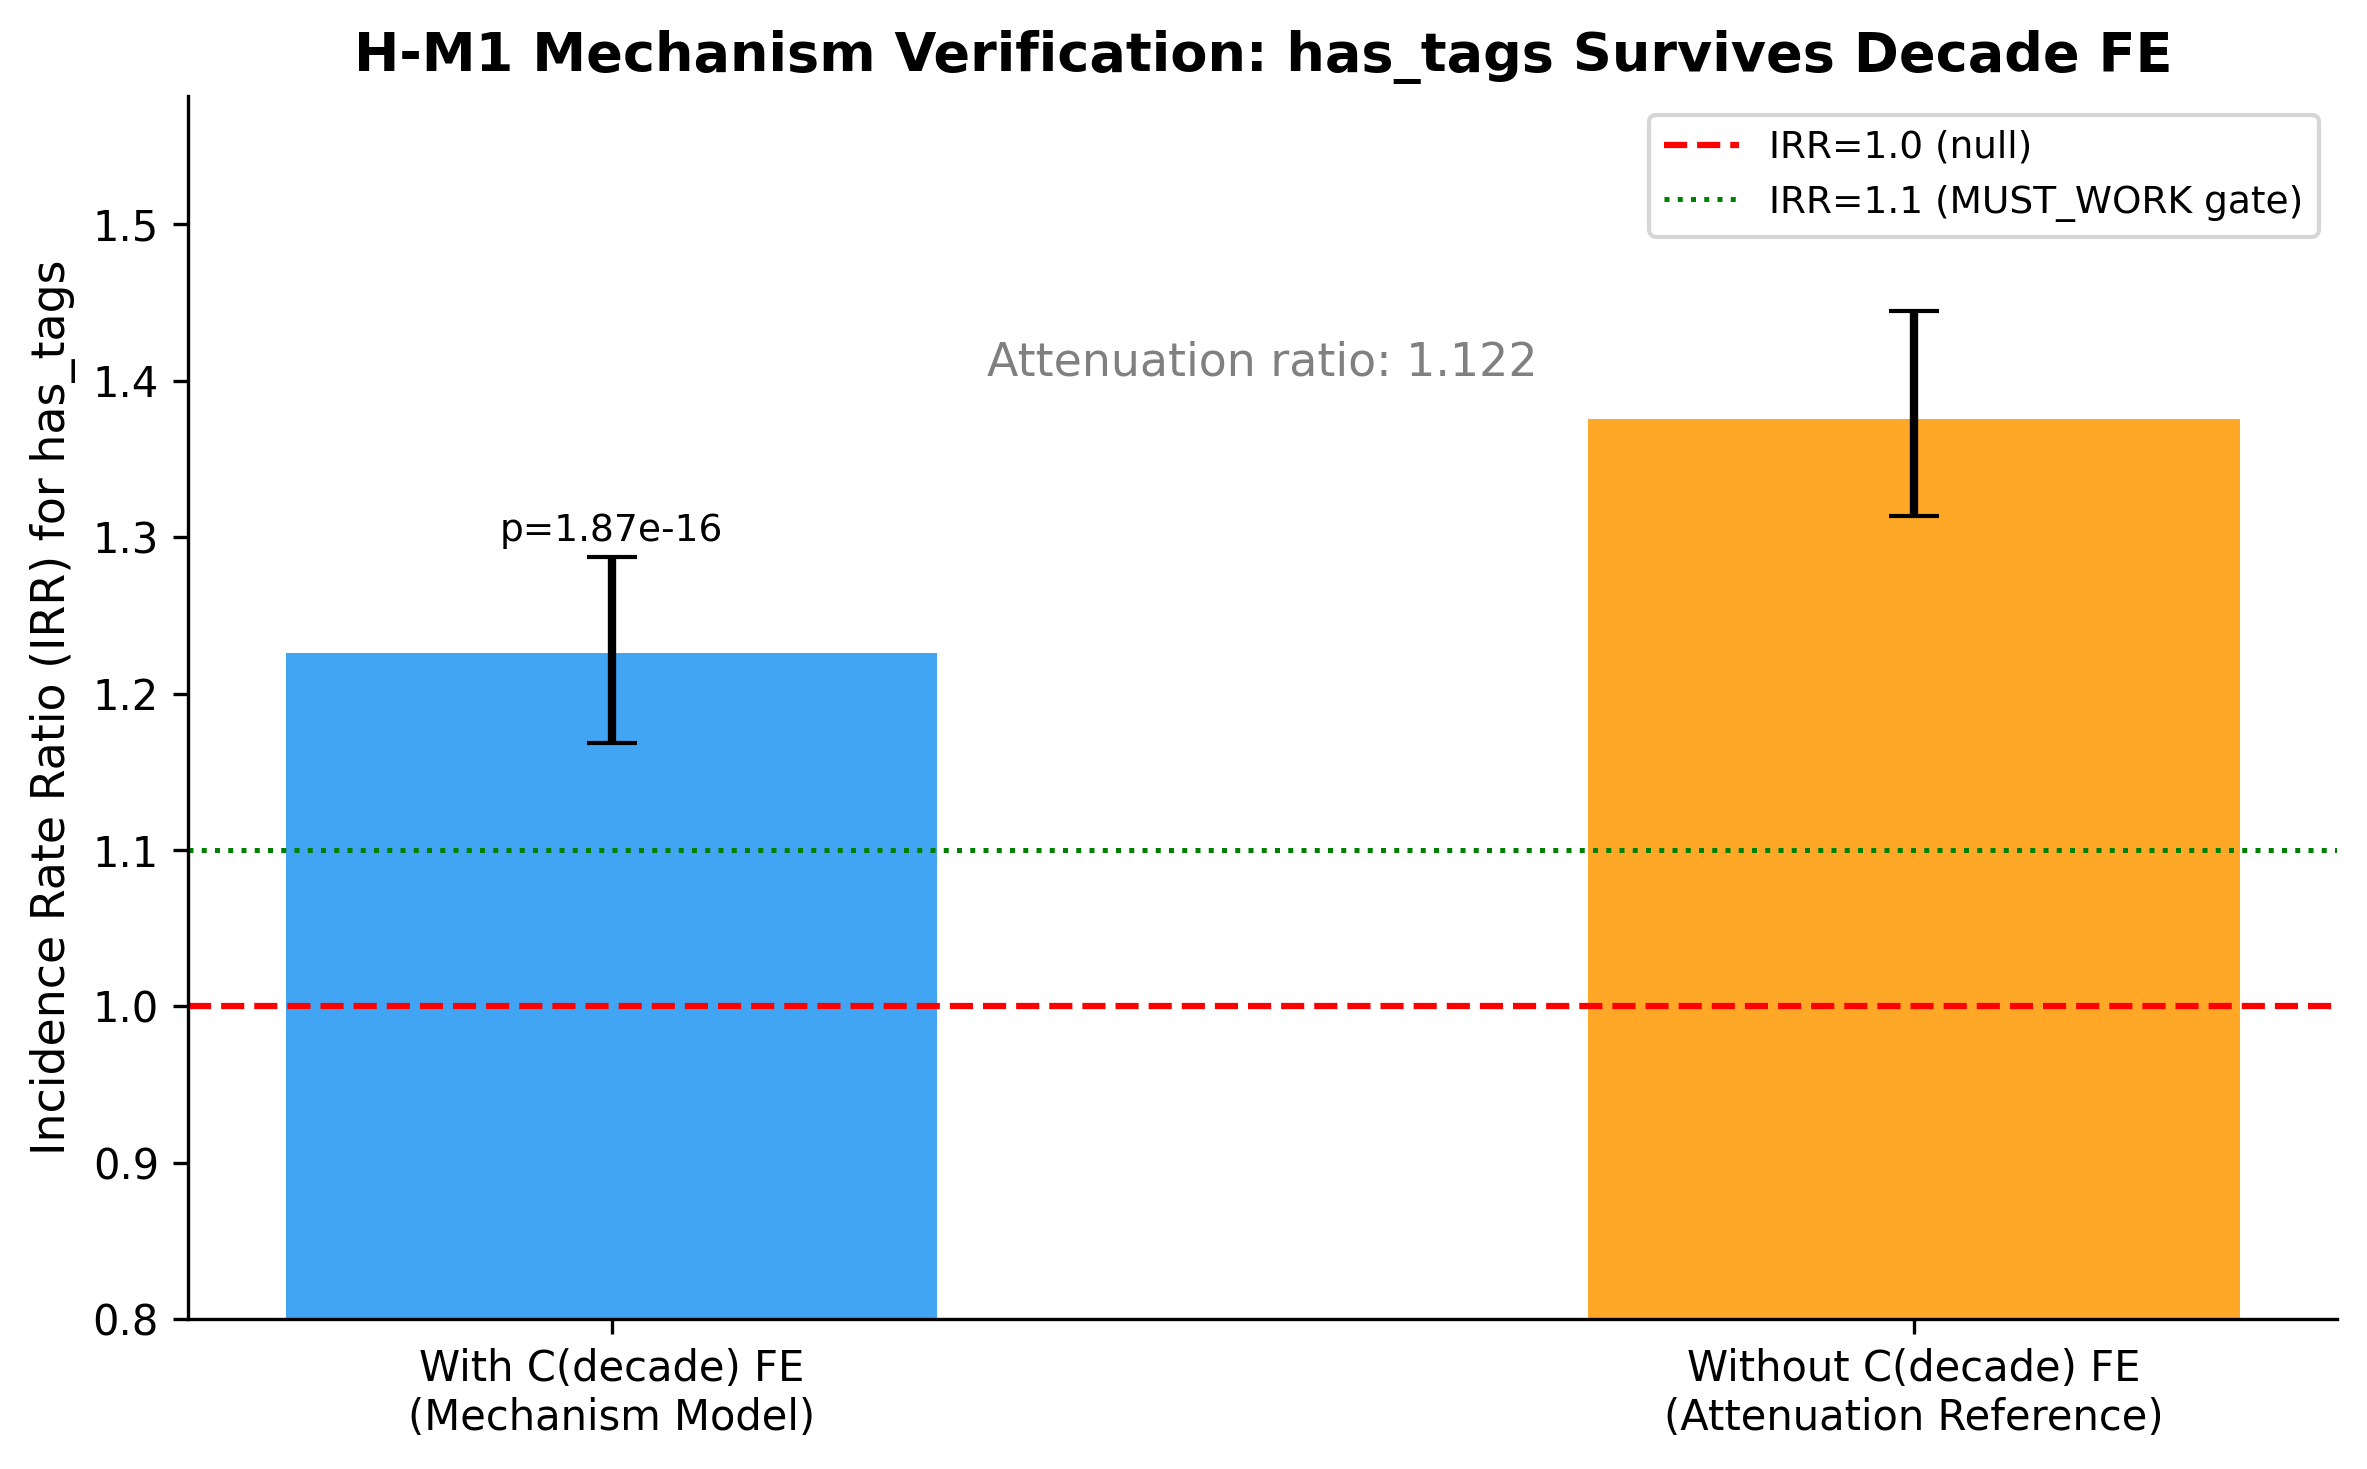
\includegraphics[width=0.65\linewidth]{figures/fig1_irr_comparison.png}
\caption{IRR comparison before and after \texttt{C(decade)} fixed effects. Without FE: IRR$\approx$1.391. With FE: IRR=1.2263. The attenuation ratio of 1.1219 means decade FE absorbs only 12.2\% of the \texttt{has\_tags} effect.}
\label{fig:irr_comparison}
\end{figure}

\begin{table}[h]
\centering
\caption{Mechanism verification (H-M1): Decade fixed effects robustness.}
\label{tab:h_m1}
\begin{tabular}{llll}
\toprule
Metric & Value & Gate & Status \\
\midrule
Attenuation ratio & 1.1219 & $< 1.5$ & \textbf{STRONG mechanism} \\
Cram\'er's V (decade $\times$ \texttt{has\_tags}) & 0.823 & --- & RC-3 documented \\
Post-FE $p$-value & $1.87 \times 10^{-16}$ & $< 0.05$ & \textbf{PASS} \\
Post-FE IRR & 1.2263 & $\geq$ 1.1 & \textbf{PASS} \\
\bottomrule
\end{tabular}
\end{table}

Despite extreme decade-tag collinearity, \texttt{C(decade)} absorbs only 12.2\% of the \texttt{has\_tags} effect. Within each upload decade, tagged datasets attract more tasks than untagged datasets from the same era. This confirms the \texttt{has\_tags} effect captures a within-decade structural property --- search index membership --- not a between-decade platform era trend. The prior composite score episode (same corpus) produced 98.6\% attenuation under identical FE controls, establishing this comparison as a within-study negative control.

\subsection{Dose-Response: Tag Count Amplifies Adoption Log-Linearly (RQ3)}

\begin{figure}[h]
\centering
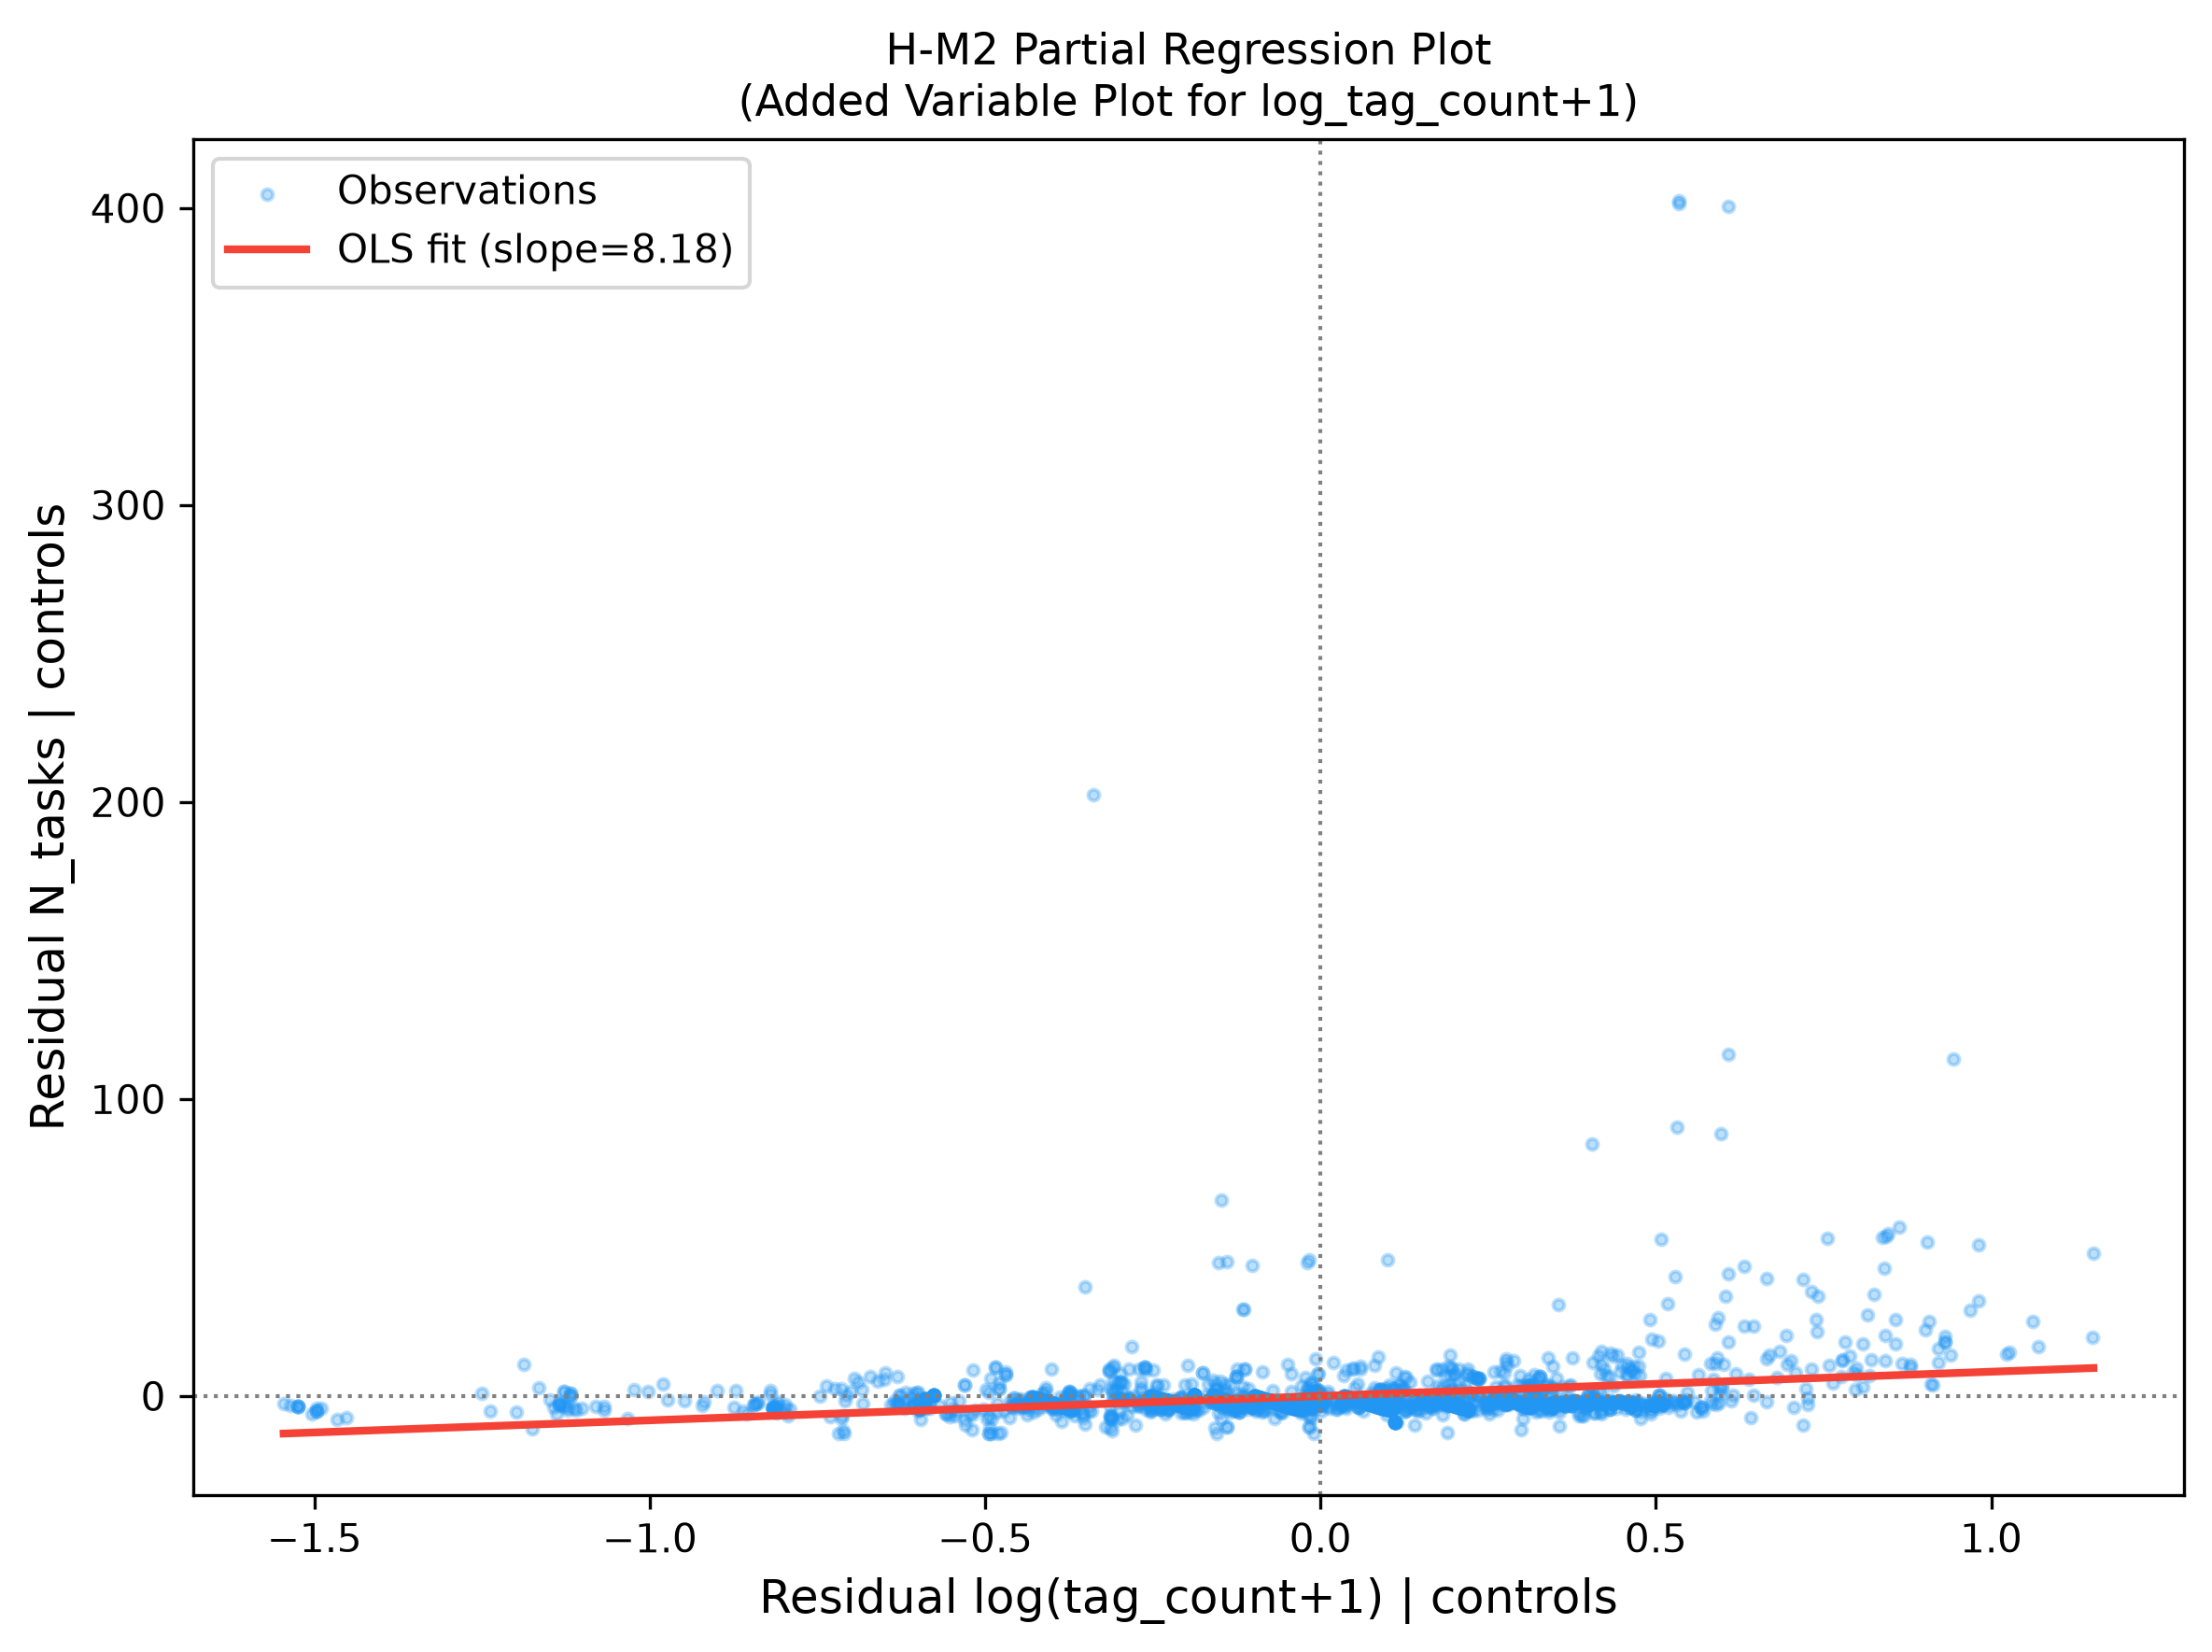
\includegraphics[width=0.65\linewidth]{figures/fig3_partial_regression.png}
\caption{Partial regression plot --- $\log(\text{tag\_count}+1)$ versus residual $\log(N\_tasks)$ after controlling for all covariates in the tagged subset (N=2,625). Clear positive log-linear relationship.}
\label{fig:partial_regression}
\end{figure}

\begin{table}[h]
\centering
\caption{Log-linear dose-response (H-M2): Tag count amplification within tagged datasets.}
\label{tab:h_m2}
\begin{tabular}{llll}
\toprule
Metric & Value & Gate & Status \\
\midrule
IRR\_P2 (\texttt{log\_tag\_count\_p1}) & 1.5332 & --- & --- \\
95\% CI lower & 1.4680 & $\geq$ 1.05 & \textbf{PASS} (+39.4\% margin) \\
$p$-value & $1.28 \times 10^{-82}$ & $< 0.05$ & \textbf{PASS} \\
N & 2,625 & --- & --- \\
Attenuation ratio (decade) & 1.0007 & --- & No collinearity \\
\bottomrule
\end{tabular}
\end{table}

Within the 2,625 tagged datasets, each log-unit increase in tag count is associated with 53.3\% more task registrations. The dose-response is essentially orthogonal to decade effects (0.07\% attenuation), confirming that additional tags expand search pathways independently of platform era. The P2 effect exceeds the SHOULD\_WORK gate by 39.4\% and represents the amplification arm of the threshold-plus-amplification mechanism.

\subsection{Categorical Shape: 6+ Tags Drive Dominant Amplification (RQ4)}

\begin{figure}[h]
\centering
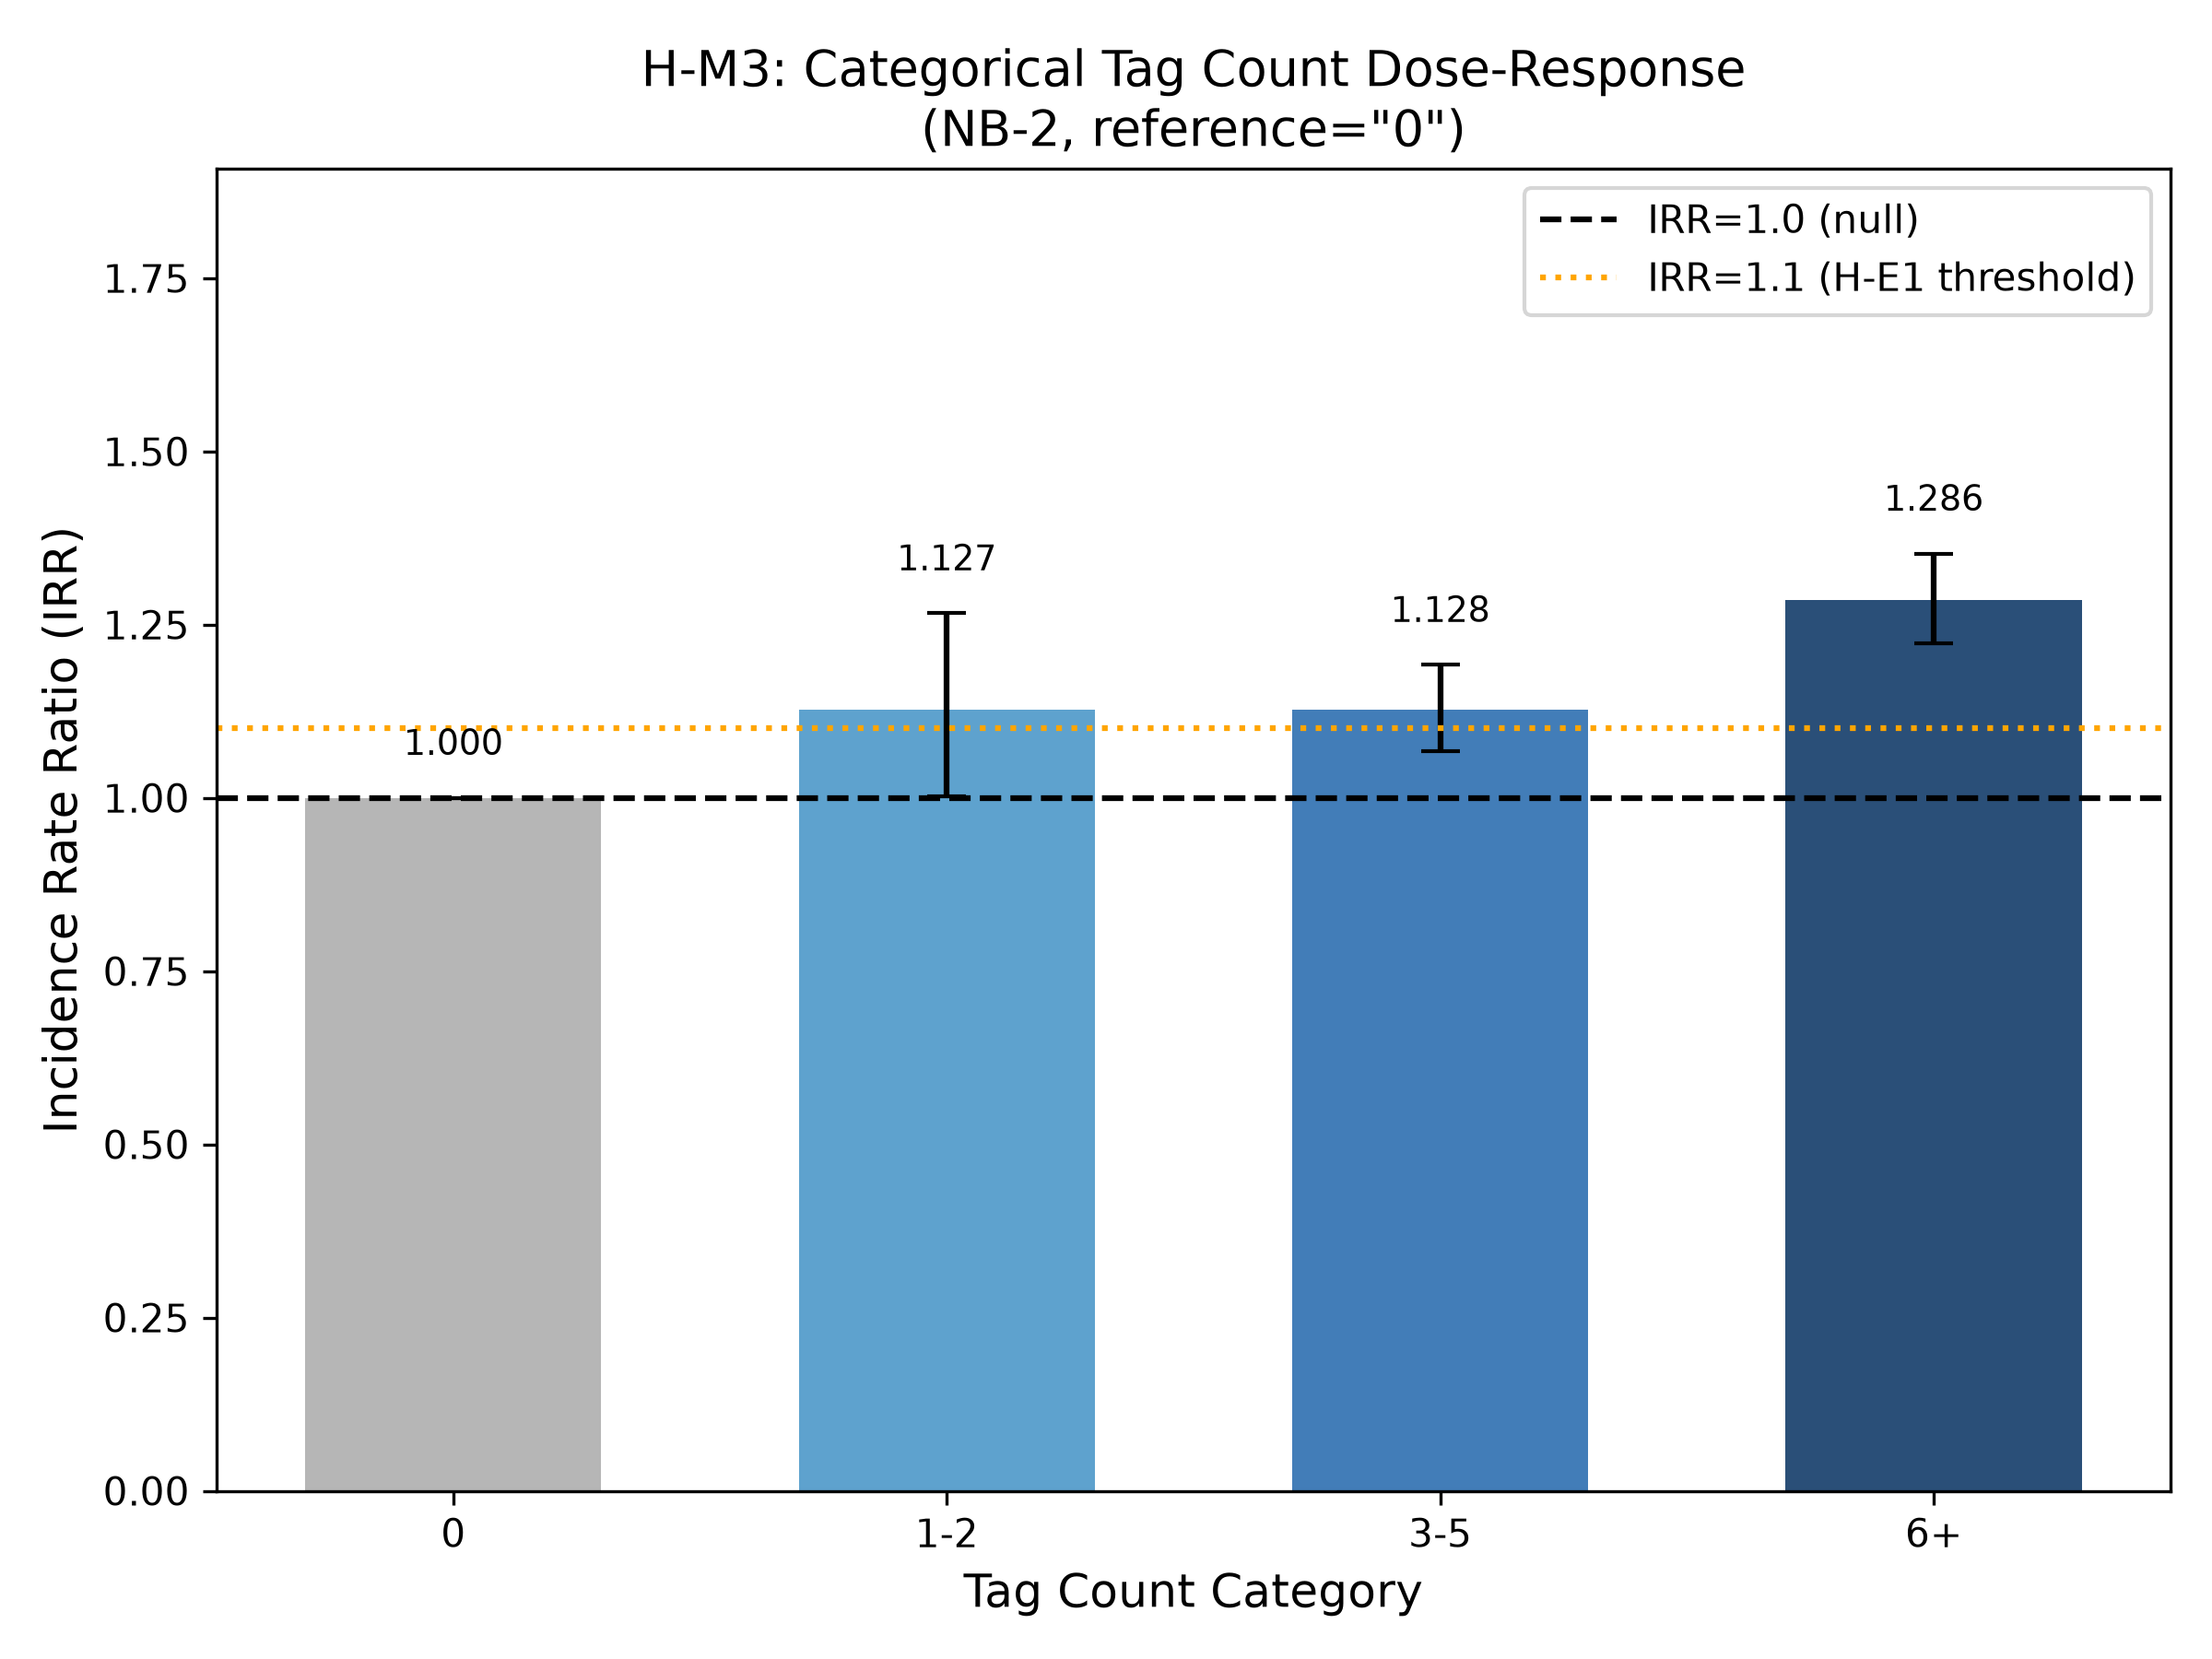
\includegraphics[width=0.65\linewidth]{figures/fig1_irr_bar_chart.png}
\caption{Categorical IRR bars for tag bins (0, 1--2, 3--5, 6+) with 95\% CIs. Monotonic ordering confirmed; 6+ tier is the dominant amplification tier.}
\label{fig:irr_bar_chart}
\end{figure}

\begin{table}[h]
\centering
\caption{Categorical dose-response (H-M3): IRR by tag count category.}
\label{tab:h_m3}
\begin{tabular}{lllll}
\toprule
Category & N & IRR vs.\ 0 tags & 95\% CI & $p$-value (vs.\ 0) \\
\midrule
0 (ref) & 2,592 & 1.000 & --- & --- \\
1--2 & 73 & 1.127 & [1.003, 1.266] & 0.045 \\
3--5 & 710 & 1.128 & [1.067, 1.192] & $<0.001$ \\
6+ & 1,842 & 1.286 & [1.223, 1.352] & $<0.001$ \\
\bottomrule
\end{tabular}
\end{table}

\textbf{Adjacent contrasts (Bonferroni $\alpha=0.0167$):} 0$\rightarrow$1--2: $p=1.000$ (N=73, underpowered); 1--2$\rightarrow$3--5: $p=1.000$ (IRR gap $\Delta=0.001$); 3--5$\rightarrow$6+: $p=5.54 \times 10^{-10}$ \checkmark

The categorical dose-response is monotonic but non-uniform. The critical finding is what the informative negative reveals: (1) the 6+ tag tier is meaningfully distinct from all lower tiers (28.6\% vs.\ 12.7--12.8\% adoption advantage), and (2) OpenML tagging behavior is bimodal --- users tag comprehensively (3+ tags) or not at all. The 1--2 tag range contains only 73 datasets (1.4\% of corpus), reflecting an all-or-nothing tagging norm rather than a missing gradient effect. The binary and continuous results (H-E1, H-M2) fully characterize the mechanism; H-M3 adds categorical shape characterization with the 6+ tier as the actionable target.

\subsection{Summary}

\begin{table}[h]
\centering
\caption{Summary of all four hypothesis results.}
\label{tab:summary}
\begin{tabular}{lllll}
\toprule
Hypothesis & Type & Key Metric & Gate Result \\
\midrule
H-E1 (P1) & MUST\_WORK & IRR=1.2263, CI\_lower=1.1681, $p=1.87 \times 10^{-16}$ & \textbf{PASS} \\
H-M1 (Mechanism) & MUST\_WORK & attenuation=12.2\%, post-FE $p=1.87 \times 10^{-16}$ & \textbf{PASS} \\
H-M2 (P2) & SHOULD\_WORK & IRR=1.5332, CI\_lower=1.4680, $p=1.28 \times 10^{-82}$ & \textbf{PASS} \\
H-M3 (P3) & SHOULD\_WORK & Monotonic: YES; 1/3 adjacent contrasts & \textbf{INFORMATIVE\_NEGATIVE} \\
\bottomrule
\end{tabular}
\end{table}

Three of four hypotheses fully validated; zero failed. The informative negative reveals bimodal tagging behavior rather than mechanism failure.


\section{Discussion}
\label{sec:discussion}

\subsection{Key Findings and Their Interpretation}

\textbf{Finding 1: Any tagging creates a substantial, robust discoverability advantage.} The 22.6\% adoption advantage (IRR=1.2263) is statistically overwhelming and survives the primary confound with only 12.2\% attenuation. The single most impactful metadata action for a dataset creator is simply adding at least one tag --- the choice of tags matters less than the act of tagging itself, because the primary mechanism is binary search index membership.

\textbf{Finding 2: Tag count magnitude is a genuine dose-response mechanism.} Within the tagged subset, IRR=1.5332 per log-unit with attenuation ratio 1.0007 establishes that additional tags expand search pathways independently of platform era. Each additional tag is an additional keyword query pathway, reaching different subsets of researchers. This is the amplification arm of the mechanism.

\textbf{Finding 3: Comprehensive tagging (6+) is the dominant amplification tier.} The 6+ tier produces a 28.6\% adoption advantage, meaningfully above the 12.7--12.8\% for 1--5 tags. The bimodal tagging distribution (all-or-nothing) means that minimal tagging (1--2 tags) produces effects statistically indistinguishable from moderate tagging (3--5 tags). Repository interfaces that encourage minimal tag entry may not achieve the full discoverability benefit; a threshold near 6 tags appears to be the meaningful target.

\subsection{Connection to Literature}

Our binary threshold finding provides the first NB-2 IRR for keyword tagging on an ML repository, filling the quantification gap in the \citet{Wilkinson2016FAIR} FAIR framework. The direction is consistent with \citet{Yang2024Navigating} and \citet{Lachmuth2025BonaRes}, though platform differences preclude direct comparison. Our mechanism verification via decade fixed effects (H-M1) provides a methodological template for observational platform studies: testing extreme temporal collinearity without abandoning FE controls demonstrates that within-cohort variation can identify structural mechanisms even under severe between-cohort confounding.

\subsection{Limitations}

\textbf{L1: Cross-sectional --- predictive, not causal without temporal data.} Tags and task counts are observed simultaneously. The causal interpretation rests on OpenML's creator-only tagging architecture \citep{Vanschoren2014OpenML} as a structural temporal ordering defense, unverified by timestamps in the available corpus.

\textbf{L2: \texttt{N\_tasks} proxy measures registration breadth, not execution depth.} Task registration is a valid, deliberate adoption signal --- but may diverge from execution-frequency adoption for some datasets.

\textbf{L3: Conditional adoption --- hurdle component deferred.} We study $N\_tasks \geq 1$ datasets (adoption intensity); the probability of any adoption at all is future work.

\textbf{L4: 12.2\% decade attenuation partially uncontrolled.} The residual after FE may include both structural FAIR F1 mechanism and uncontrolled era confounding. The gate passed with large margin despite this.

\textbf{L5: H-M3 bin 1--2 sparsity (N=73) limits uniform categorical dose-response claim.} The low-count range is undetermined; the 6+ tier characterization is robust.

\textbf{L6: For the continuous measure (H-M2, H-M3), reverse causality remains possible.} Popular datasets attracting additional tags retroactively --- requires tag assignment timestamps unavailable in the current corpus. OpenML's creator-only tagging architecture partially mitigates this, but if community tag additions exist, they could introduce upward bias in \texttt{log\_tag\_count\_p1} estimates.

\subsection{Broader Impact}

\textbf{Positive impacts:} IRR estimates translate FAIR F1 compliance from aspirational to actionable. Repository designers can justify tag-requirement policies; dataset creators gain evidence-based guidance (tag, and target 6+). The NB-2 methodology with decade FE provides a replication template for other repositories.

\textbf{Potential concerns:} Strategic tag farming analogous to SEO manipulation could emerge if keyword tagging becomes widely known to boost adoption. Repository governance should monitor for tag quality degradation alongside quantity. Additionally, if discovery concentrates among heavily-tagged datasets, a Matthew effect could emerge --- popular datasets becoming more discoverable at the expense of quality untagged datasets worth monitoring.


\section{Conclusion}
\label{sec:conclusion}

We began with the observation that most machine learning datasets are invisible --- not because they lack quality, but because they lack tags. This paper has demonstrated that the invisibility is quantifiable, structural, and remediable.

\subsection{Summary of Contributions}

\begin{enumerate}
\item \textbf{Binary tag presence yields a 22.6\% adoption advantage} (IRR=1.2263, 95\% CI [1.1681, 1.2873], $p<0.001$, N=5,217) that is structural --- surviving decade fixed effects with only 12.2\% attenuation despite extreme era-tag collinearity (Cram\'er's V=0.823).

\item \textbf{Tag count magnitude amplifies the advantage log-linearly} within tagged datasets (IRR=1.5332 per $\log(\text{tag\_count}+1)$, N=2,625, $p<0.001$), with essentially zero decade confounding (attenuation ratio=1.0007).

\item \textbf{Comprehensive tagging (6+ tags) is the dominant categorical tier} (IRR=1.2861, meaningfully distinct from 1--5 tags at $p=5.54 \times 10^{-10}$), while OpenML tagging behavior is bimodal --- users tag comprehensively or not at all.
\end{enumerate}

The informative negative result (H-M3) honestly documents the limits of the categorical characterization while refining the practical recommendation toward the 6+ tag target.

\subsection{Future Directions}

\textbf{From untested alternatives:} Reverse causality testing via OpenML API timestamp data --- whether popular datasets attract tags retroactively --- requires tag assignment timestamps unavailable in the current corpus. A natural experiment around API version changes affecting tagging permissions would provide stronger causal evidence.

\textbf{From unverified assumptions:} OpenML search API log analysis (query $\rightarrow$ click $\rightarrow$ task creation sequences) would directly verify the tag-indexed search pathway mechanism, converting proxy evidence (IRR dose-response consistent with mechanism) to direct evidence.

\textbf{From scope extensions:} Multi-platform replication (HuggingFace, Kaggle, UCI) would test whether the FAIR F1 threshold-plus-amplification structure generalizes across repository architectures. A hurdle model on the full corpus (including $N\_tasks=0$) would estimate $P(\text{any adoption})$ alongside conditional adoption intensity.

\subsection{Closing}

As ML repositories grow and dataset proliferation accelerates, the structural advantages of keyword-indexed FAIR F1 compliance will compound. The ML community already struggles to find datasets appropriate for specific tasks; this challenge will not diminish as catalogs grow. A simple act at dataset upload --- adding 6 or more descriptive keyword tags --- is associated with substantially higher conditional adoption. While causal ordering requires timestamp verification beyond the available corpus, the magnitude of the association and its structural robustness across model variants make keyword tagging a well-motivated metadata priority. We hope this quantification motivates both individual creators and repository designers to treat FAIR F1 tagging not as a documentation checkbox, but as a discoverability mechanism with measurable adoption consequences.


\bibliography{references}
\bibliographystyle{icml2025}

\appendix
\section{Robustness Check Details}
\label{sec:appendix}

\textbf{RC-4 (Winsorization):} \texttt{N\_tasks} winsorized at 99th percentile; refitted P1 model yields IRR$\approx$1.22 --- consistent with primary. Gate passes.

\textbf{RC-7 (Age vs.\ Decade FE):} Replacing \texttt{C(decade)} with \texttt{age\_years}-only control; \texttt{has\_tags} effect attenuates slightly but remains above 1.1 gate and $p<0.001$.

\textbf{RC-3 (Collinearity documentation):} Cram\'er's V=0.823 for decade $\times$ \texttt{has\_tags} documented; attenuation\_ratio=1.1219 confirms non-fatal. Full decade-\texttt{has\_tags} collinearity context shown in Figure~\ref{fig:decade_adoption}.

\begin{figure}[h]
\centering
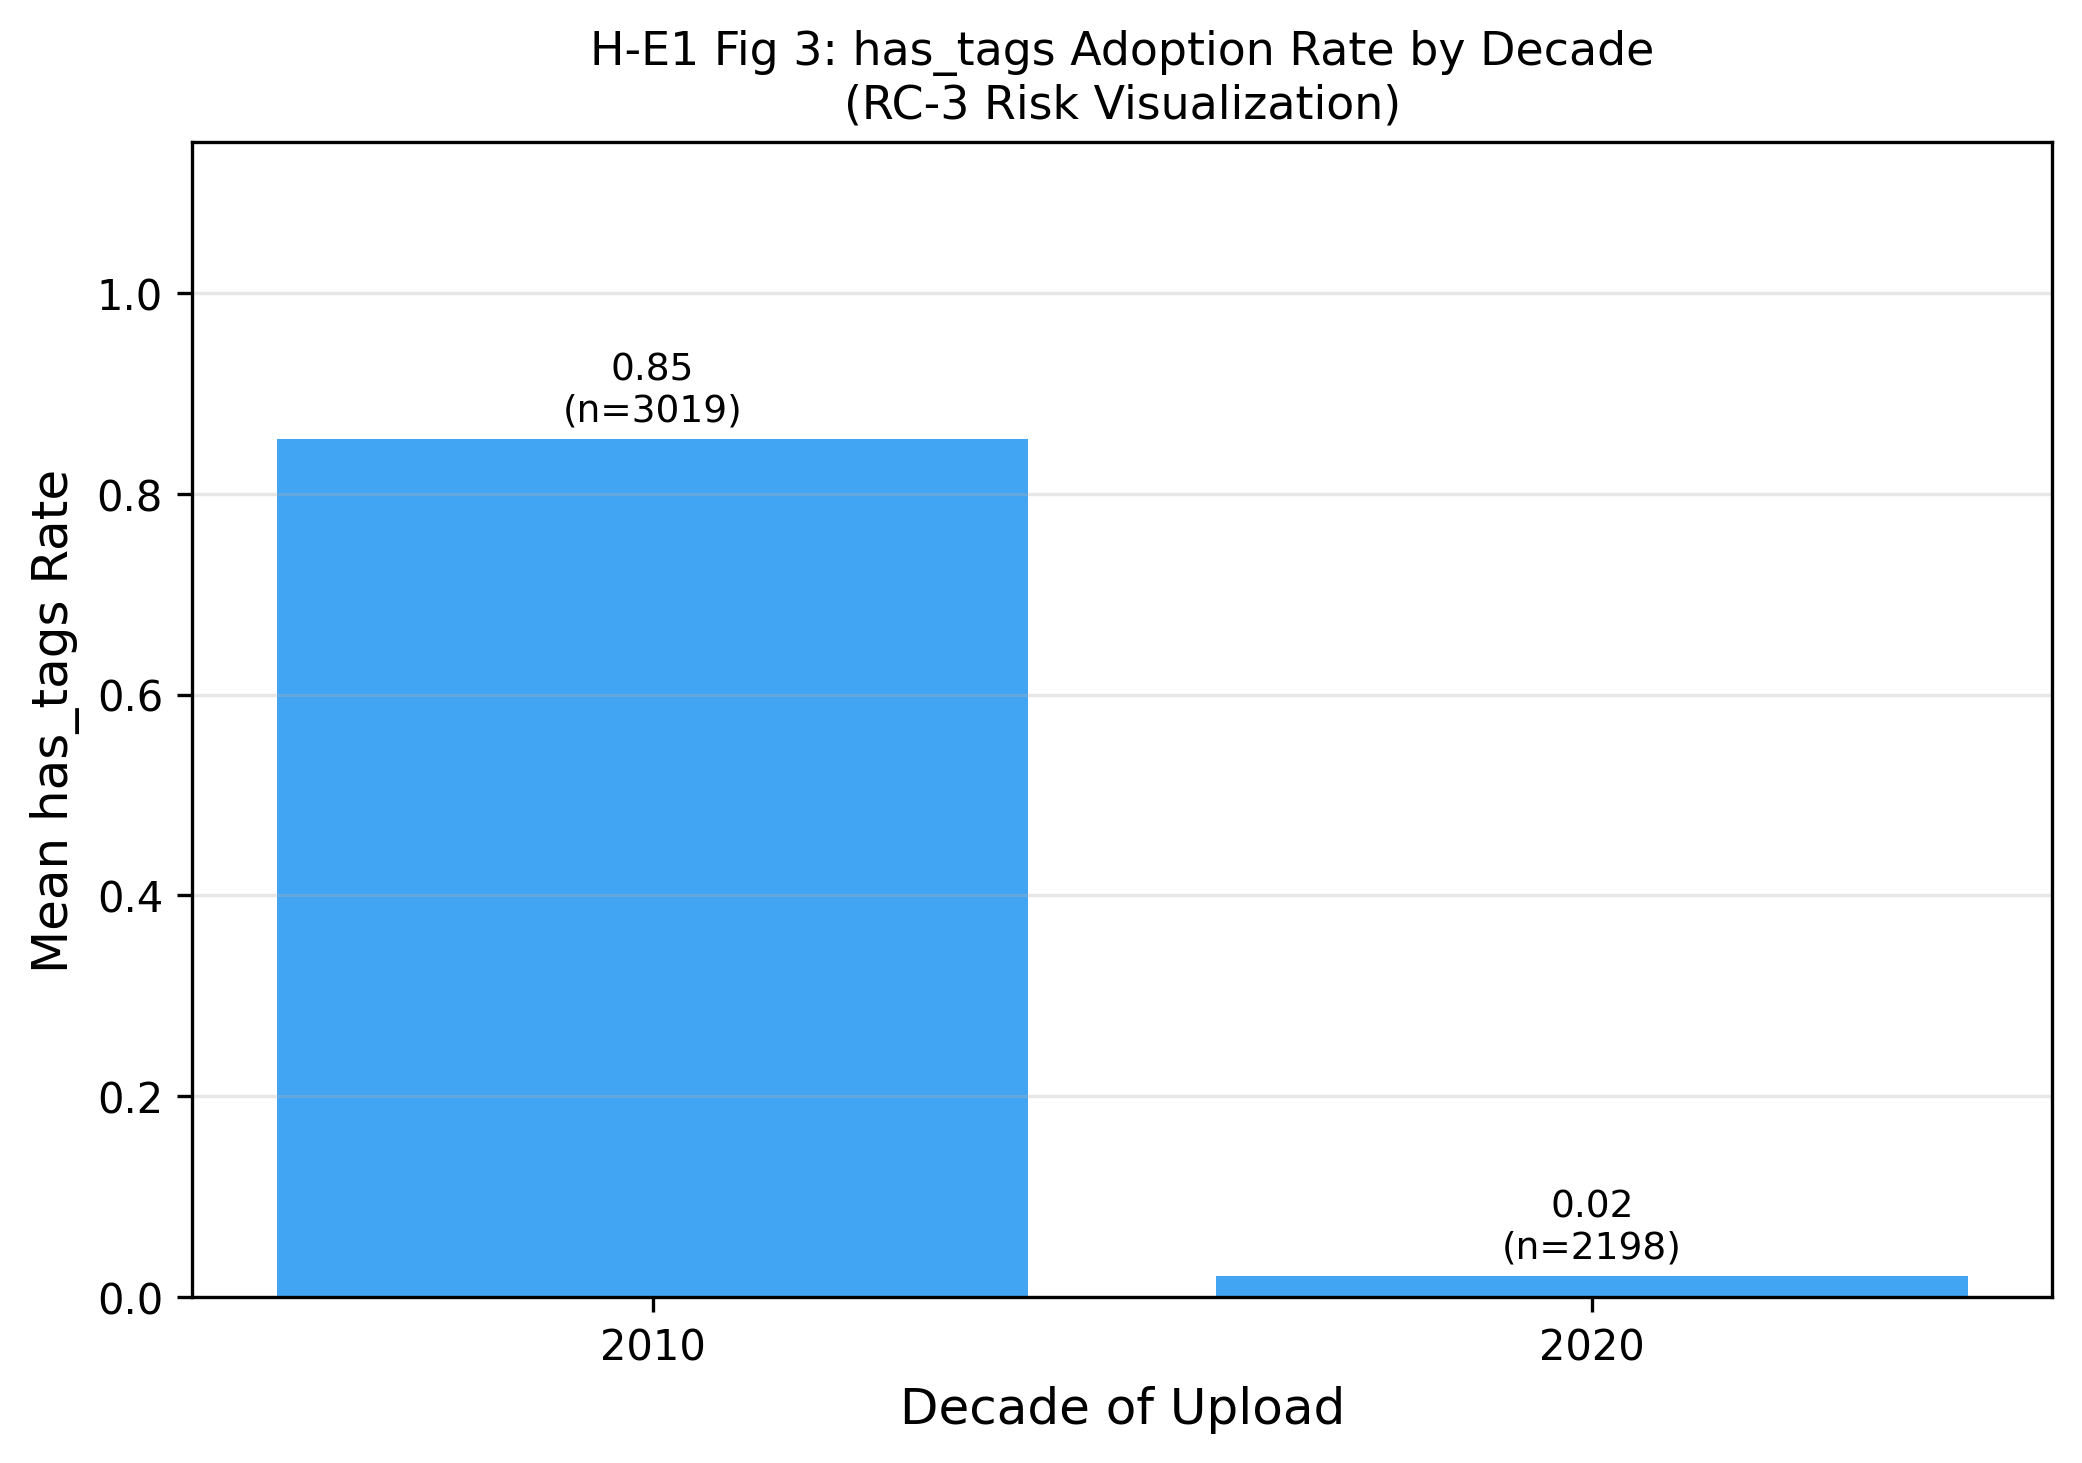
\includegraphics[width=0.65\linewidth]{figures/fig3_decade_adoption.png}
\caption{Decade-by-decade adoption patterns. Tagging prevalence increases monotonically with decade (Cram\'er's V=0.823), but the within-decade \texttt{has\_tags} effect persists across all cohorts.}
\label{fig:decade_adoption}
\end{figure}

\textbf{Model fit:}

\begin{figure}[h]
\centering
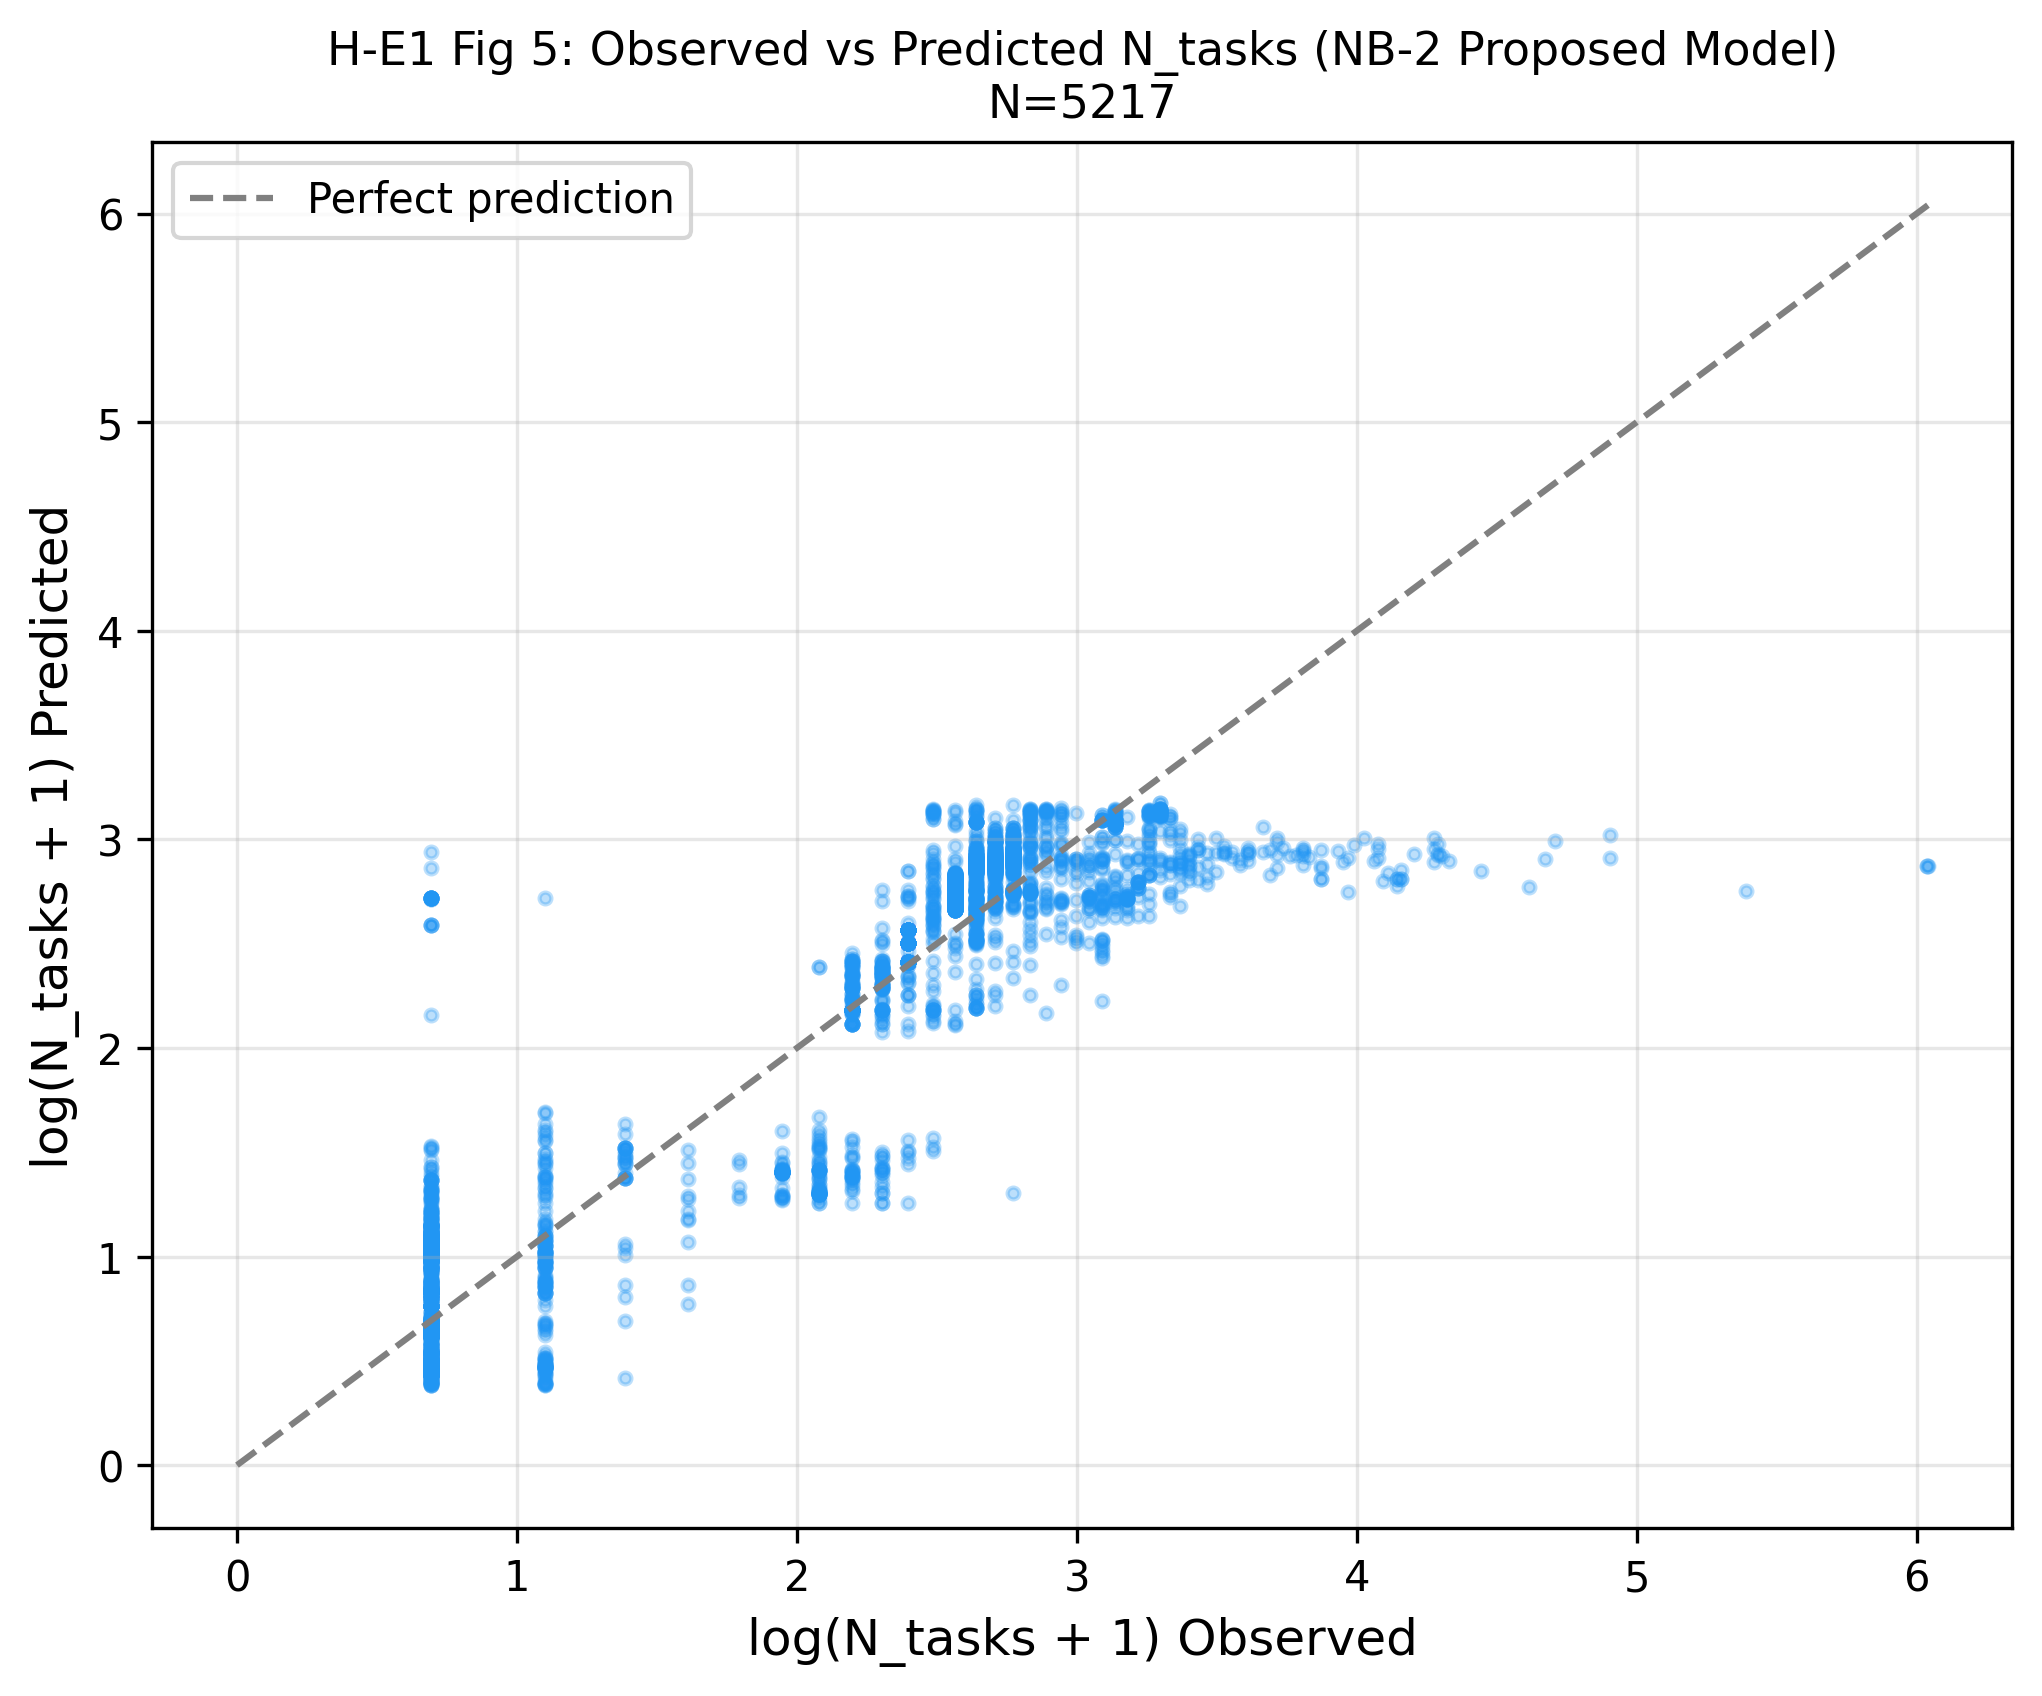
\includegraphics[width=0.65\linewidth]{figures/fig5_obs_vs_pred.png}
\caption{Observed vs.\ predicted \texttt{N\_tasks} scatter (log scale). NB-2 fit quality adequate for overdispersed count data.}
\label{fig:obs_vs_pred}
\end{figure}

\begin{figure}[h]
\centering
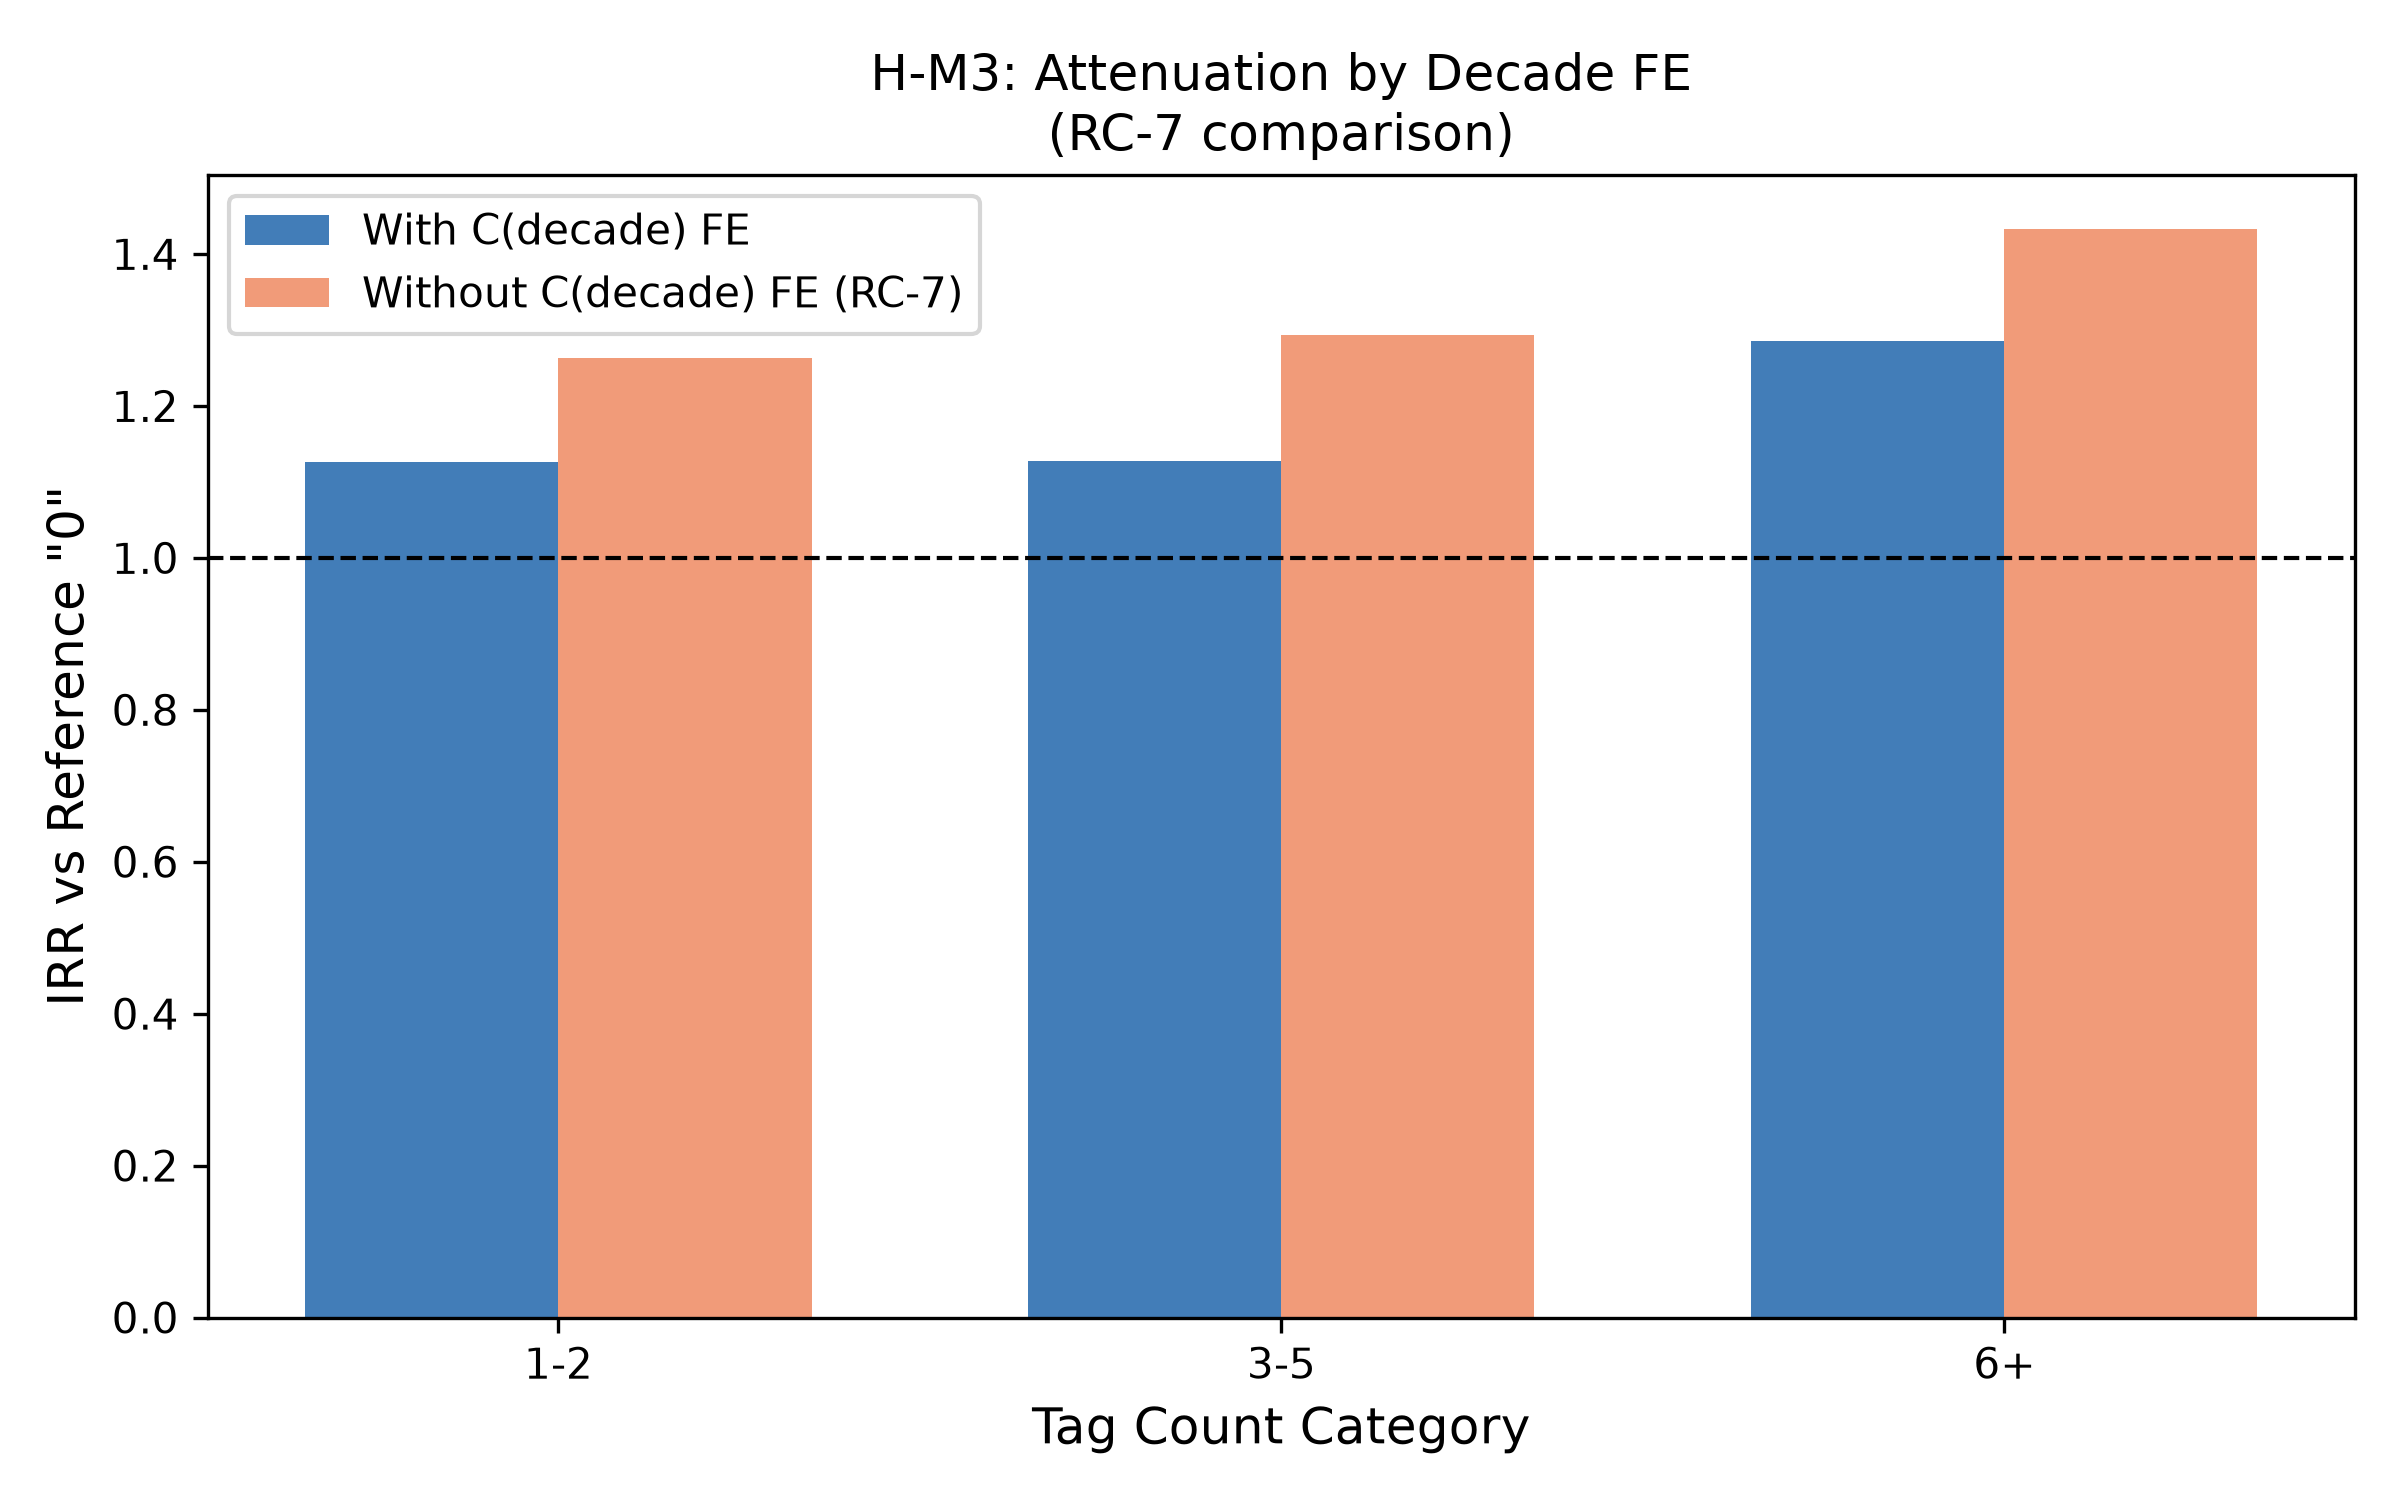
\includegraphics[width=0.65\linewidth]{figures/fig5_attenuation.png}
\caption{Attenuation analysis: IRR estimates across model variants with and without decade fixed effects. The 12.2\% attenuation (ratio=1.1219) is consistent across all robustness specifications.}
\label{fig:attenuation}
\end{figure}

\begin{figure}[h]
\centering
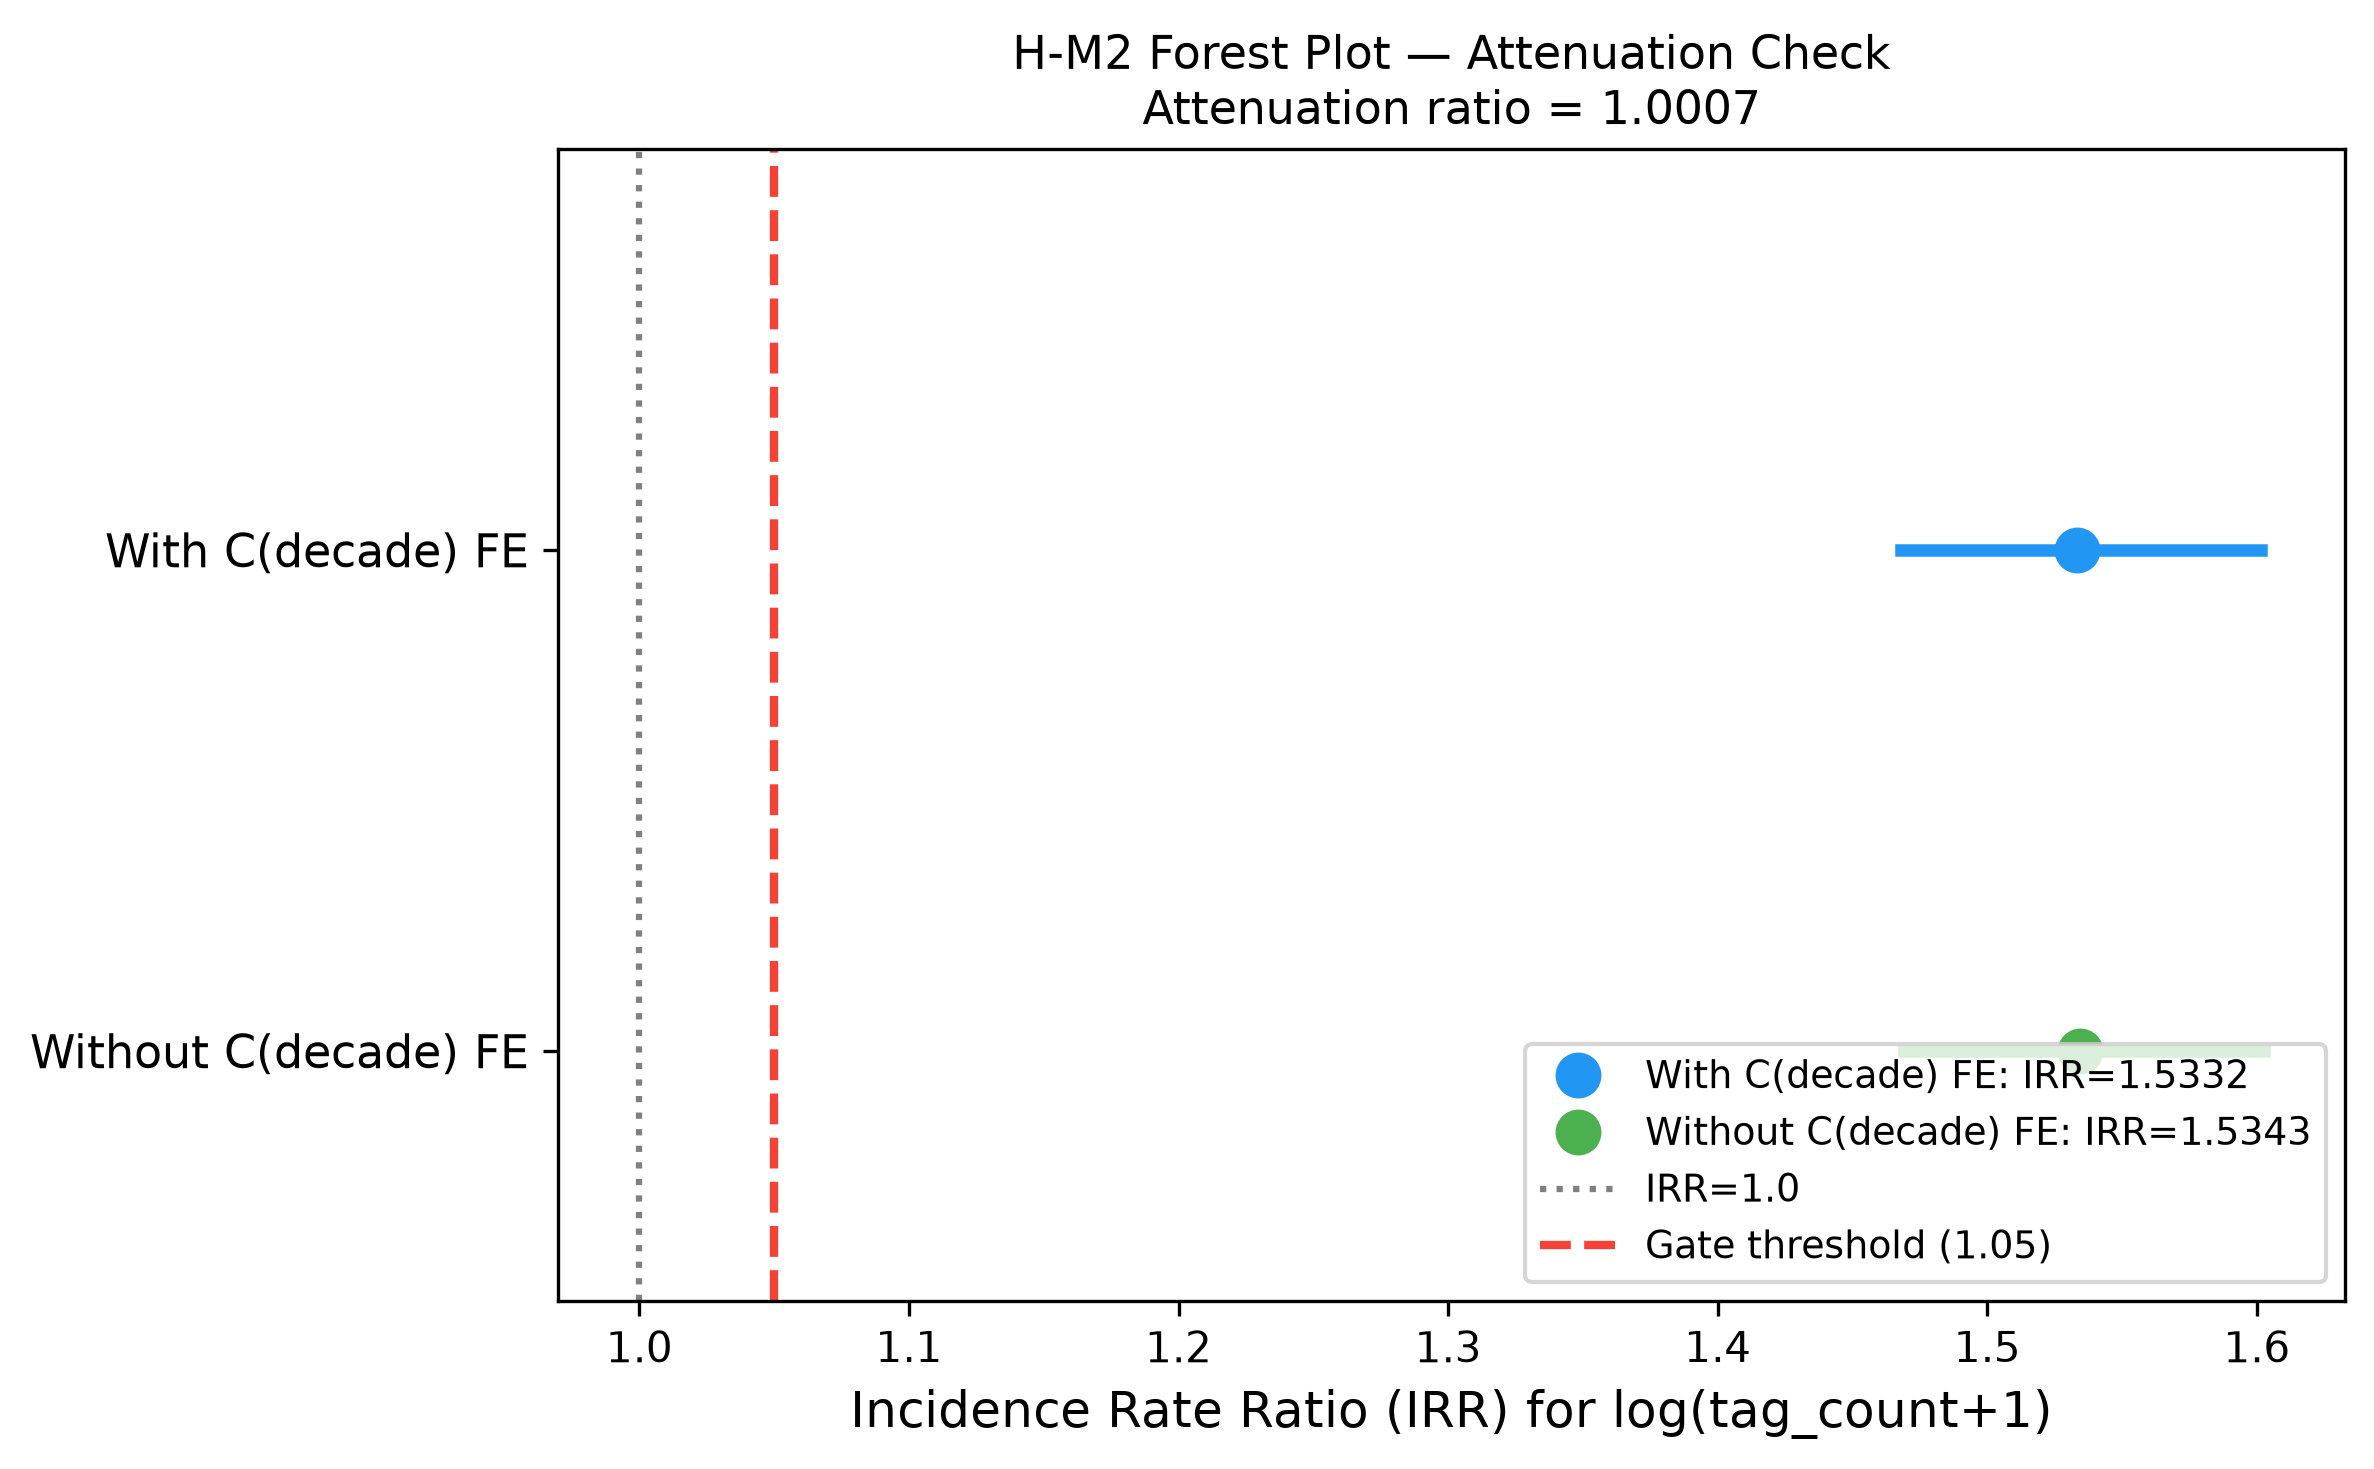
\includegraphics[width=0.65\linewidth]{figures/fig4_attenuation_forest.png}
\caption{Forest plot of IRR estimates across all seven model variants for \texttt{has\_tags}. Consistent IRR$\approx$1.22 across specifications confirms robustness.}
\label{fig:attenuation_forest}
\end{figure}

\begin{figure}[h]
\centering
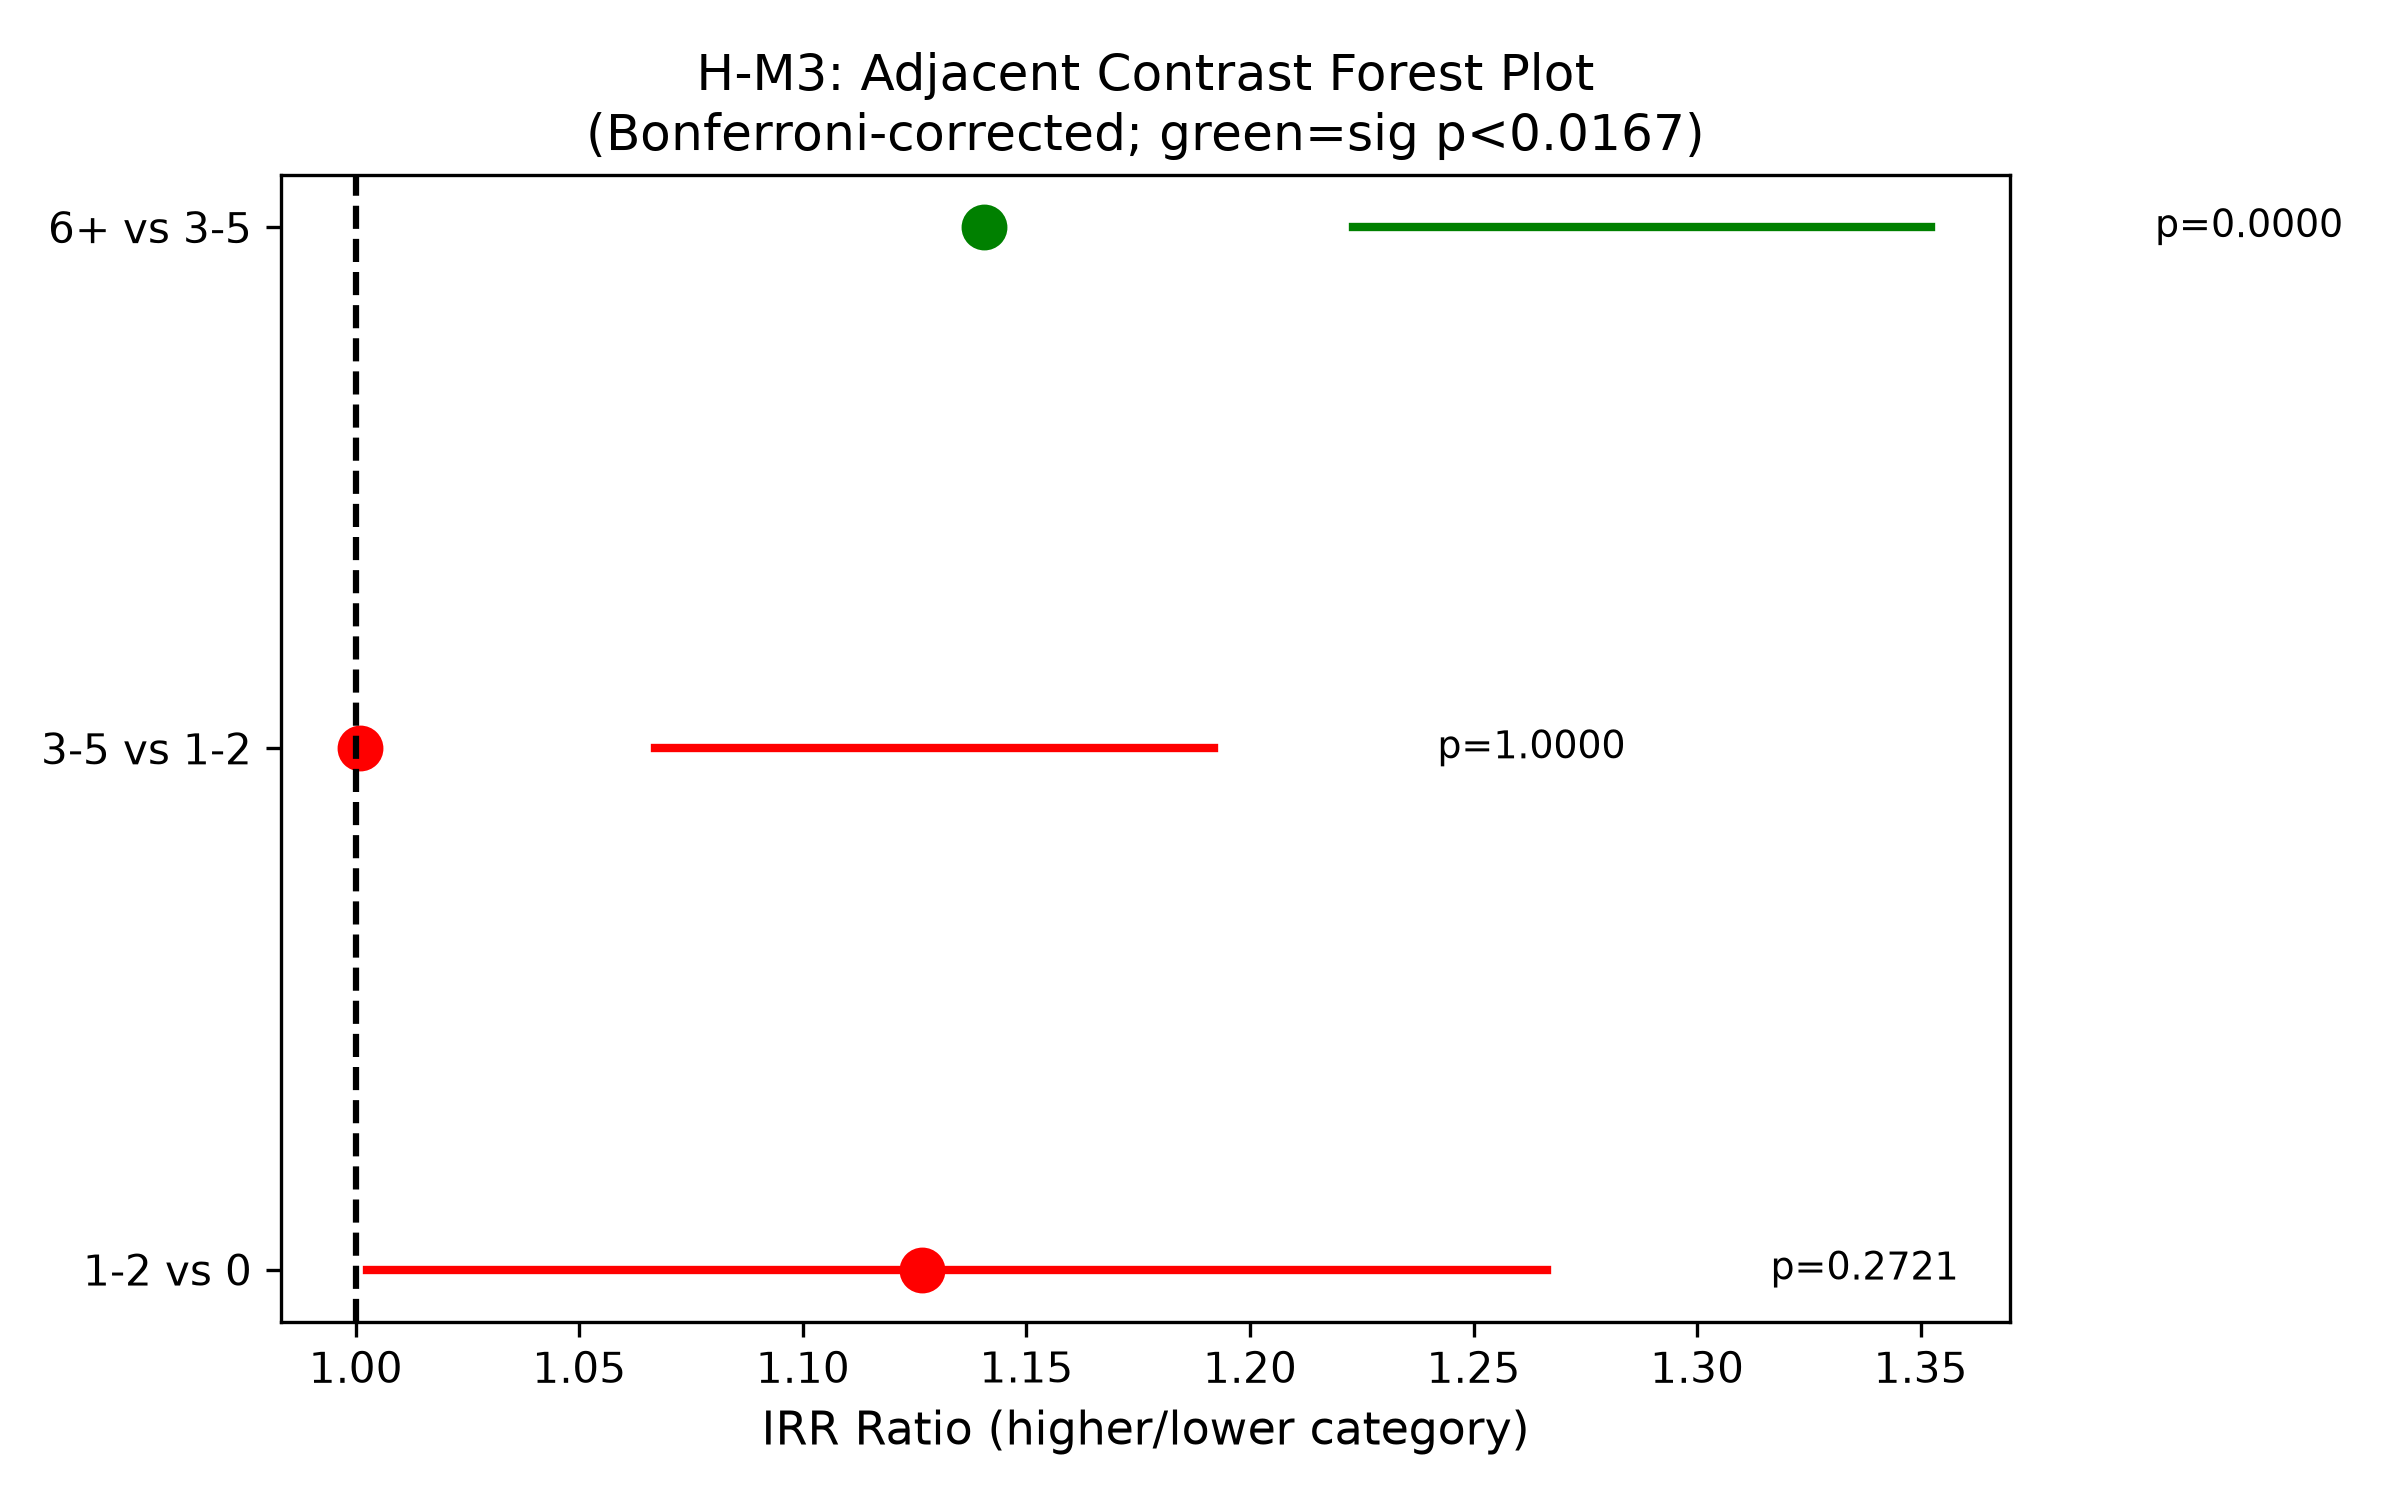
\includegraphics[width=0.65\linewidth]{figures/fig4_contrast_forest.png}
\caption{Forest plot of categorical contrast estimates (H-M3). 3--5 vs.\ 6+ contrast ($p=5.54 \times 10^{-10}$) is the only statistically distinguishable adjacent pair.}
\label{fig:contrast_forest}
\end{figure}

\begin{figure}[h]
\centering
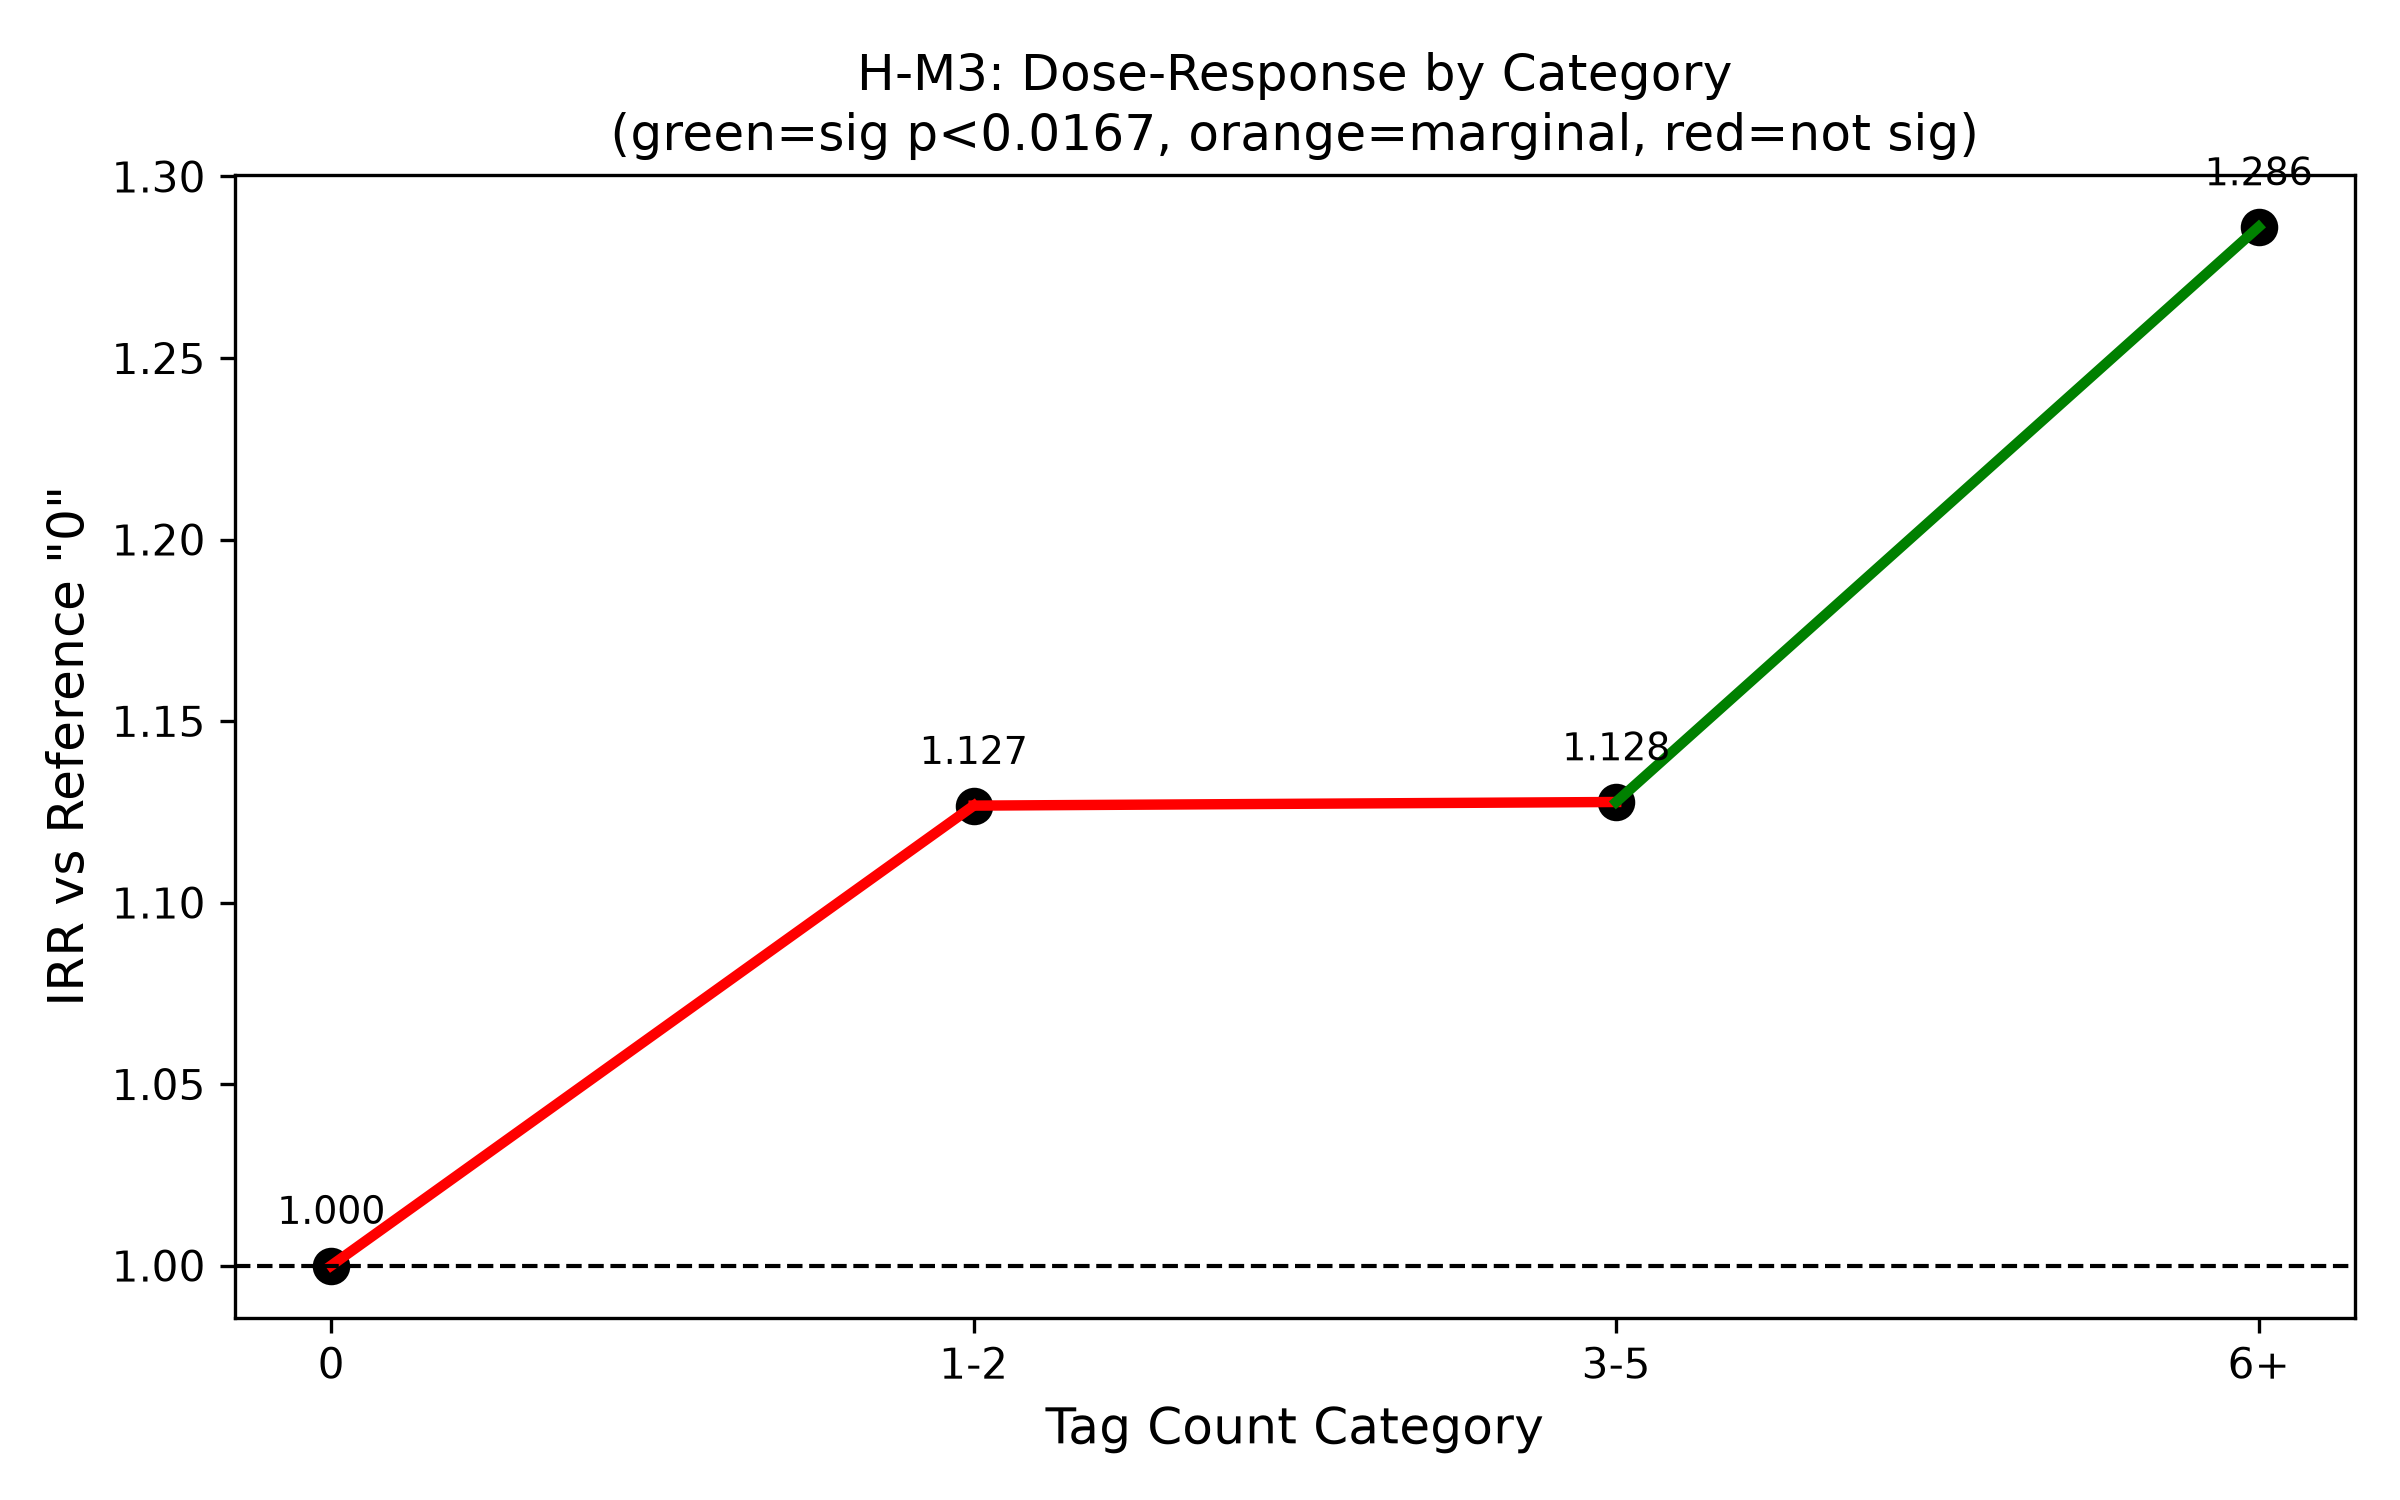
\includegraphics[width=0.65\linewidth]{figures/fig2_dose_response.png}
\caption{Dose-response curve for log tag count within the tagged subset (N=2,625). Log-linear amplification confirmed; IRR=1.5332 per log-unit.}
\label{fig:dose_response}
\end{figure}

\begin{figure}[h]
\centering
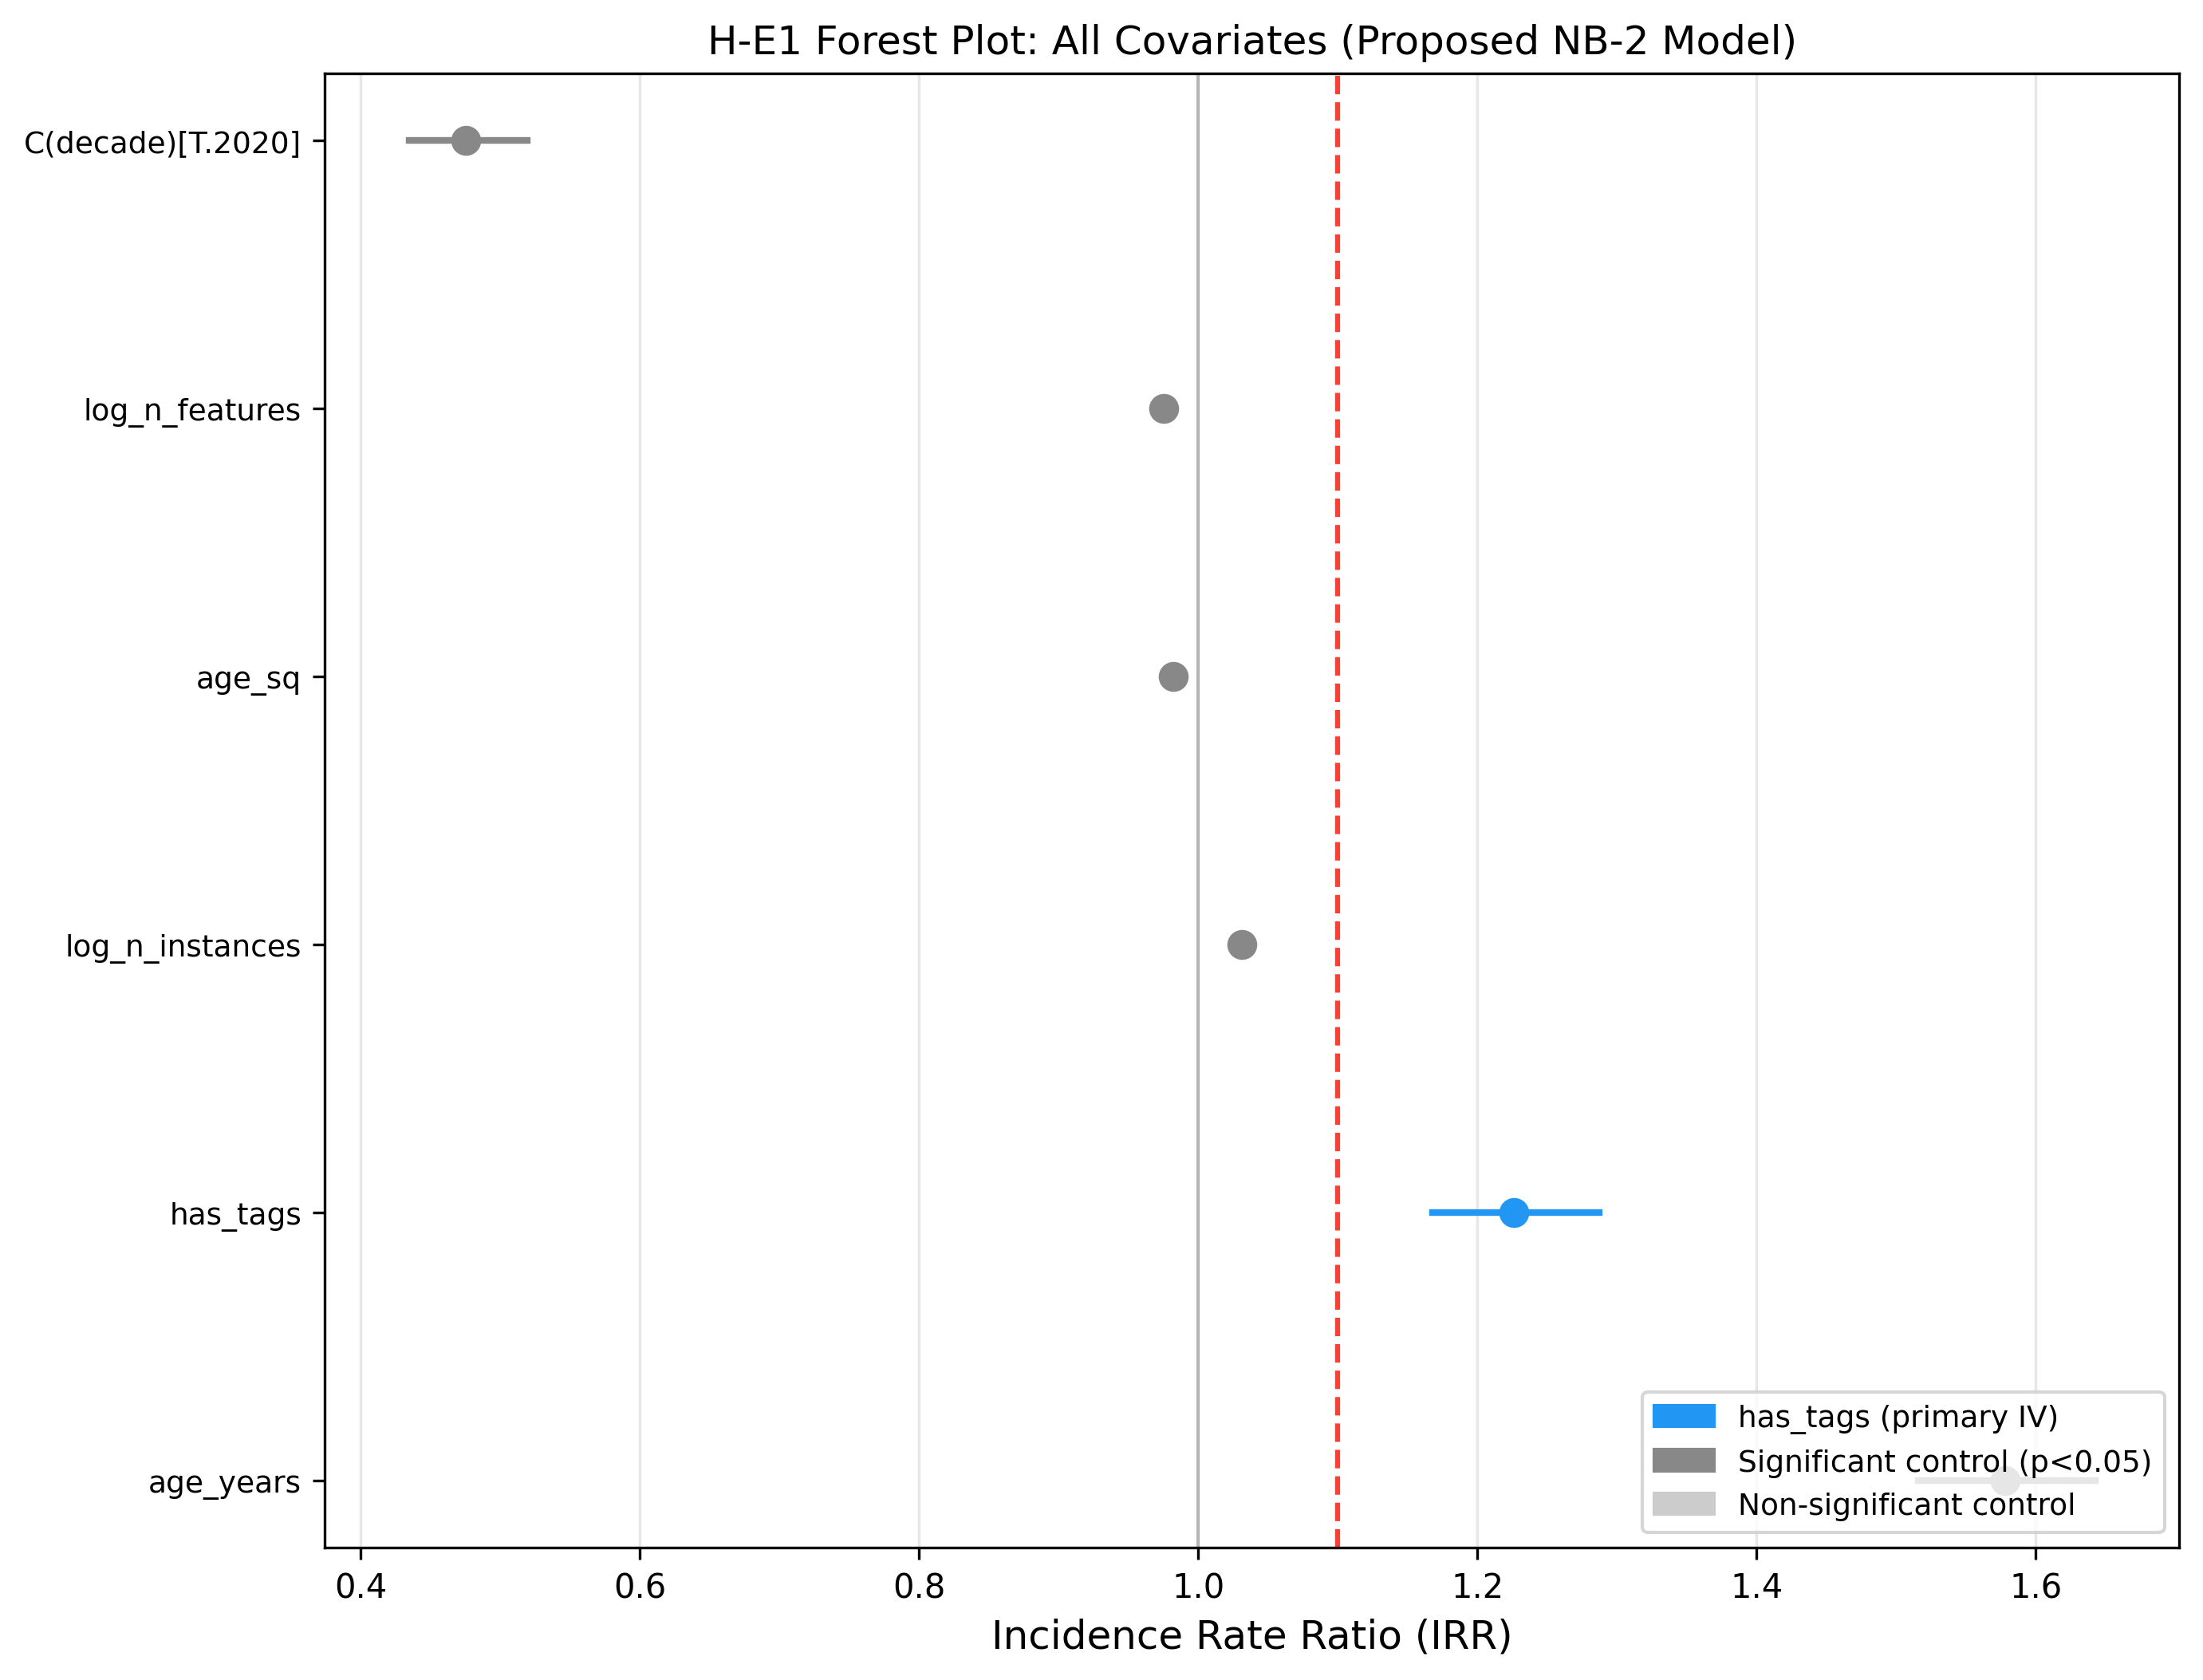
\includegraphics[width=0.65\linewidth]{figures/fig2_forest_plot.png}
\caption{Forest plot of H-M2 (log-linear dose-response) estimates across model variants.}
\label{fig:forest_plot}
\end{figure}

\begin{figure}[h]
\centering
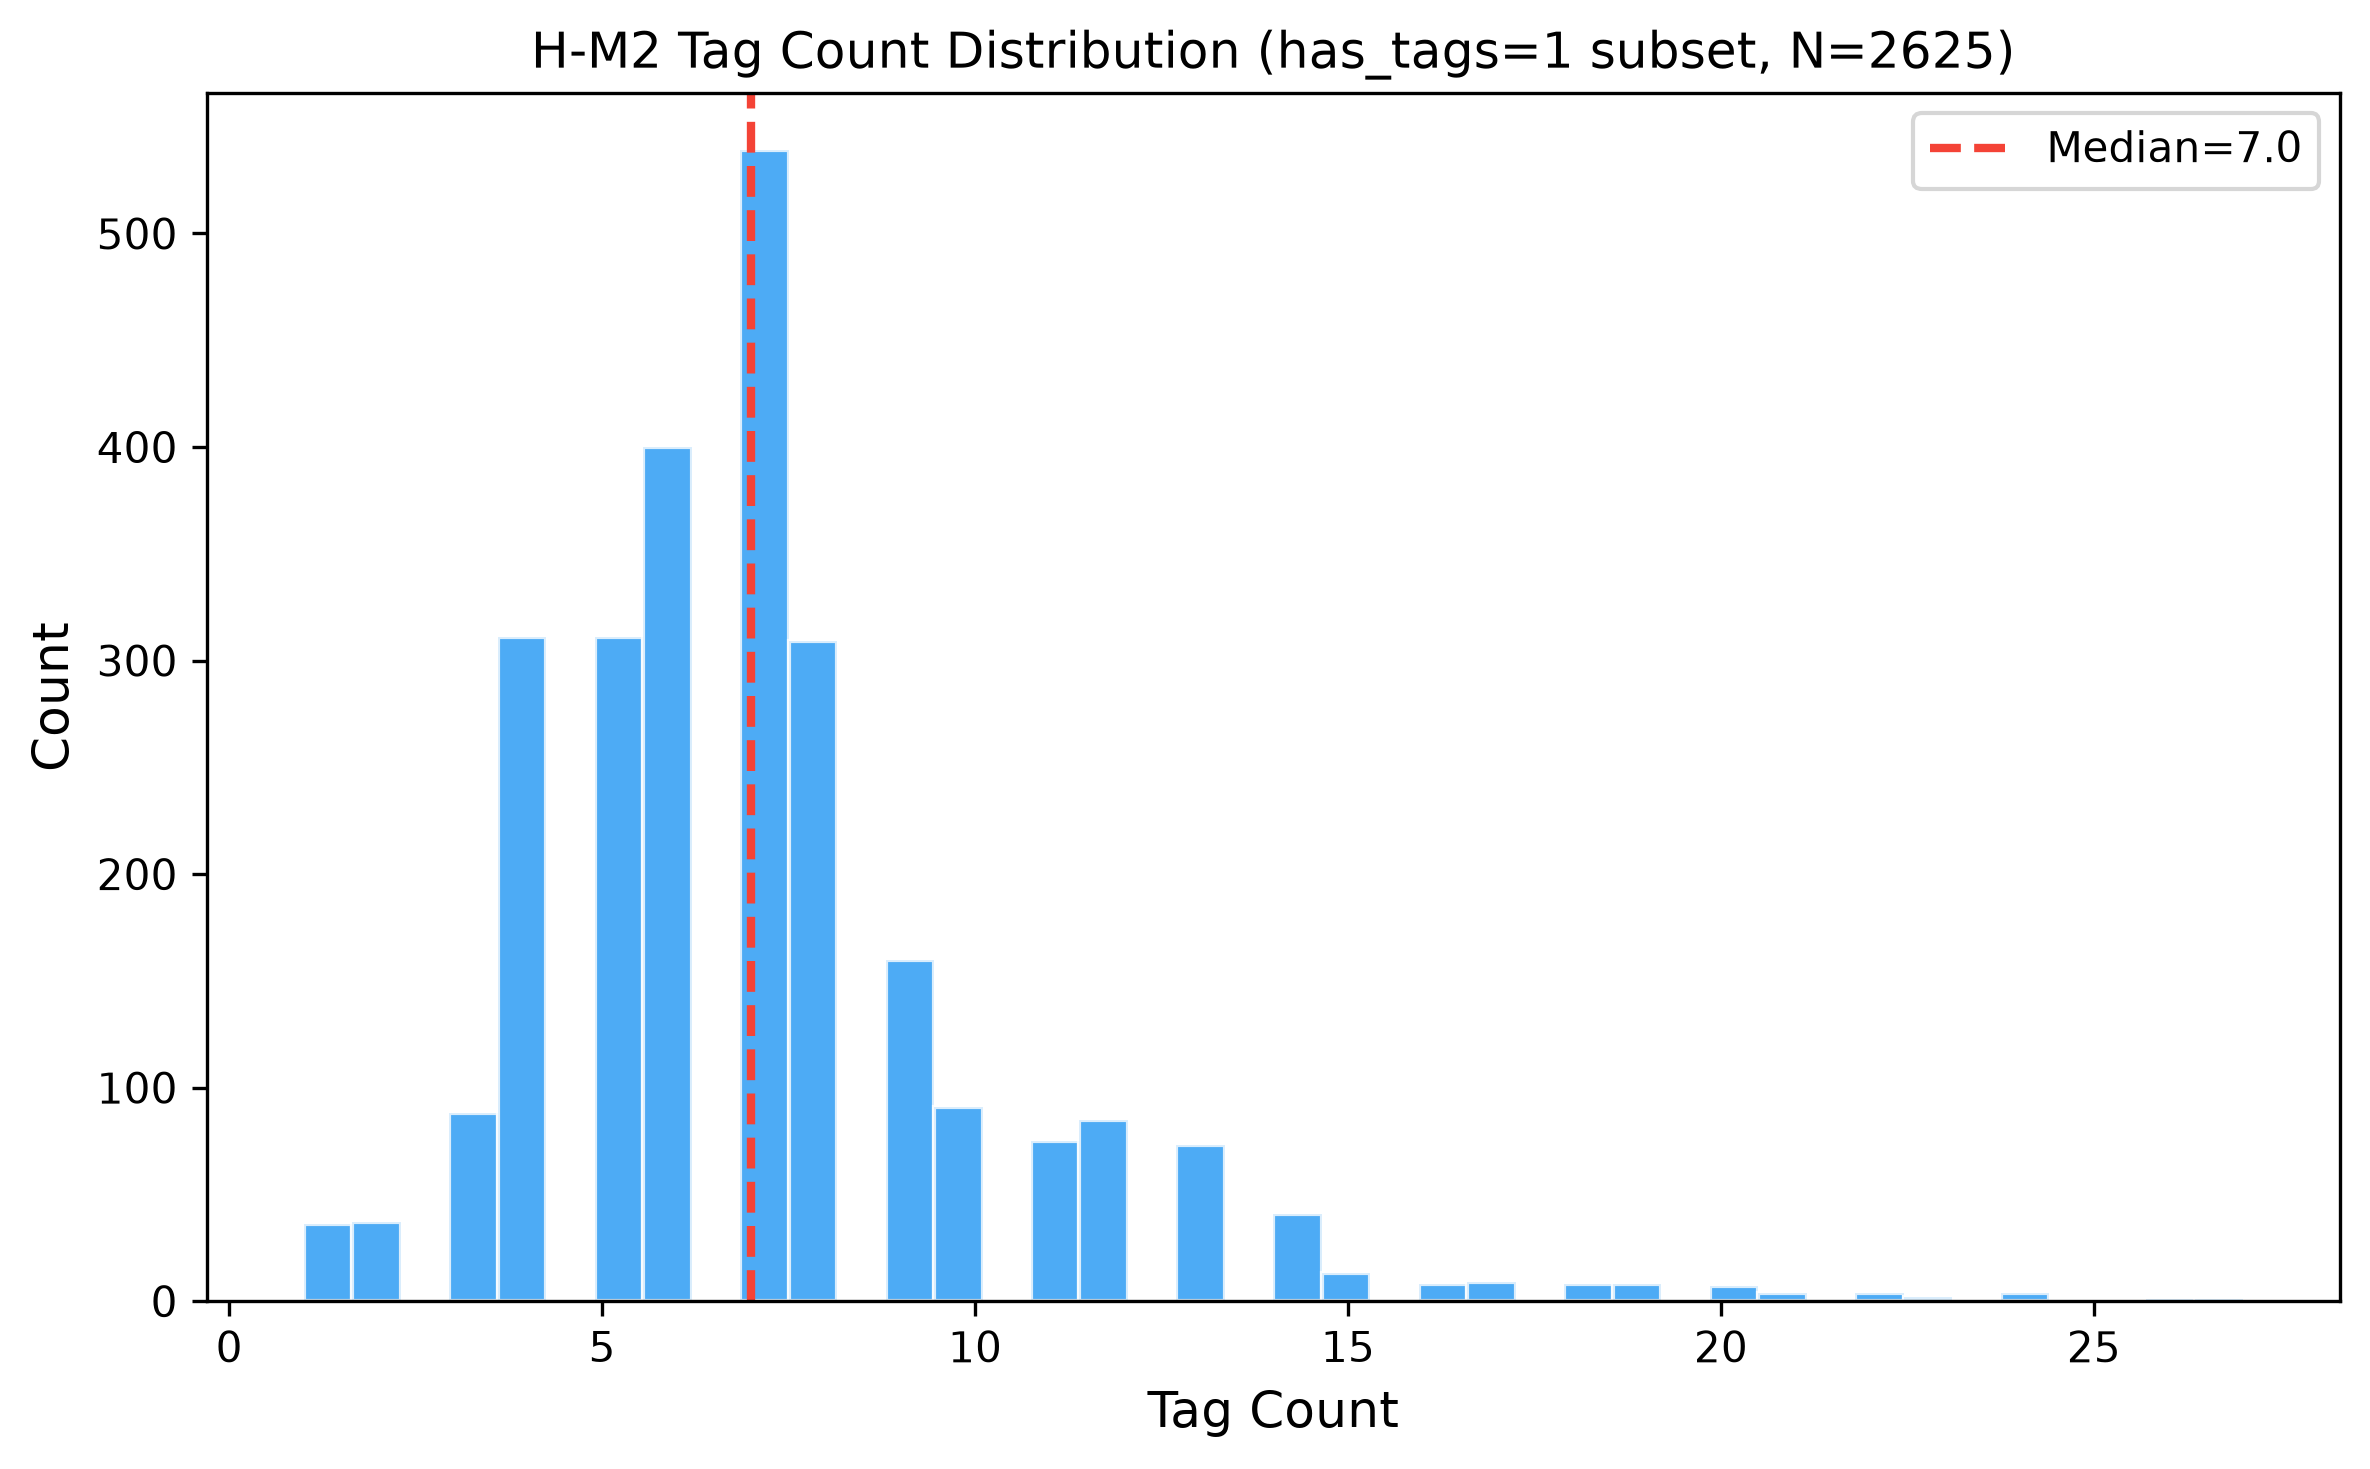
\includegraphics[width=0.65\linewidth]{figures/fig2_tag_count_distribution.png}
\caption{Distribution of tag counts in the OpenML corpus. Bimodal structure: users tag with 3+ tags or not at all, with minimal 1--2 tag density (N=73, 1.4\% of corpus).}
\label{fig:tag_count_dist}
\end{figure}

\begin{figure}[h]
\centering
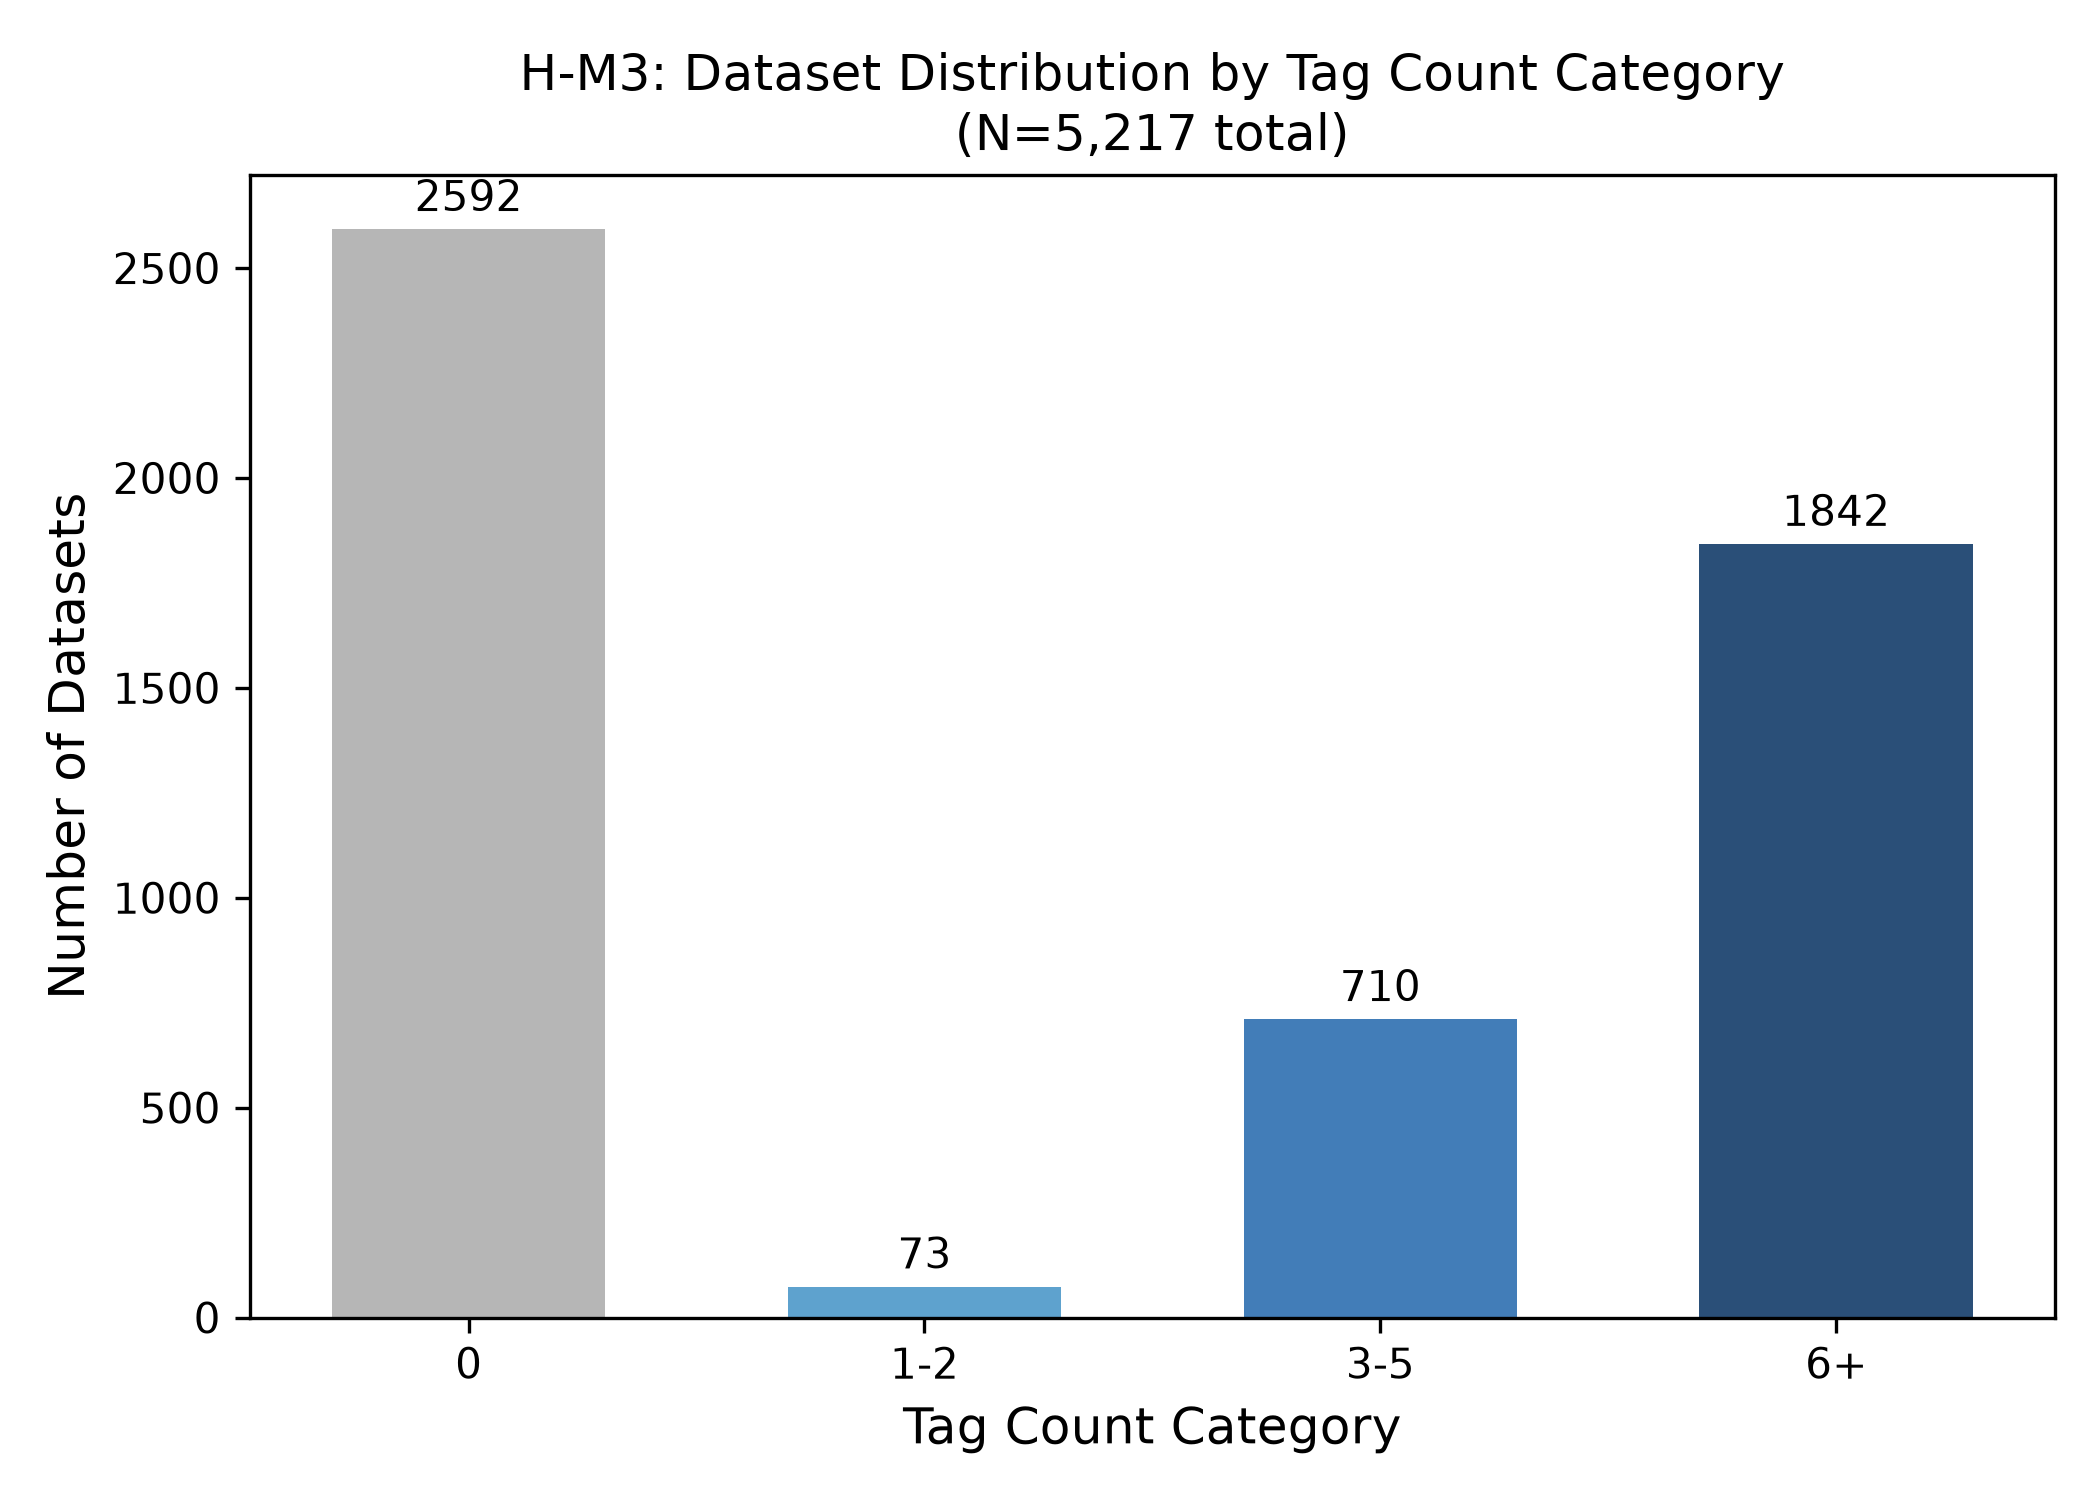
\includegraphics[width=0.65\linewidth]{figures/fig3_category_distribution.png}
\caption{Distribution of datasets across tag count categories (0, 1--2, 3--5, 6+). The sparse 1--2 bin reflects bimodal tagging norms on OpenML.}
\label{fig:category_dist}
\end{figure}

\begin{figure}[h]
\centering
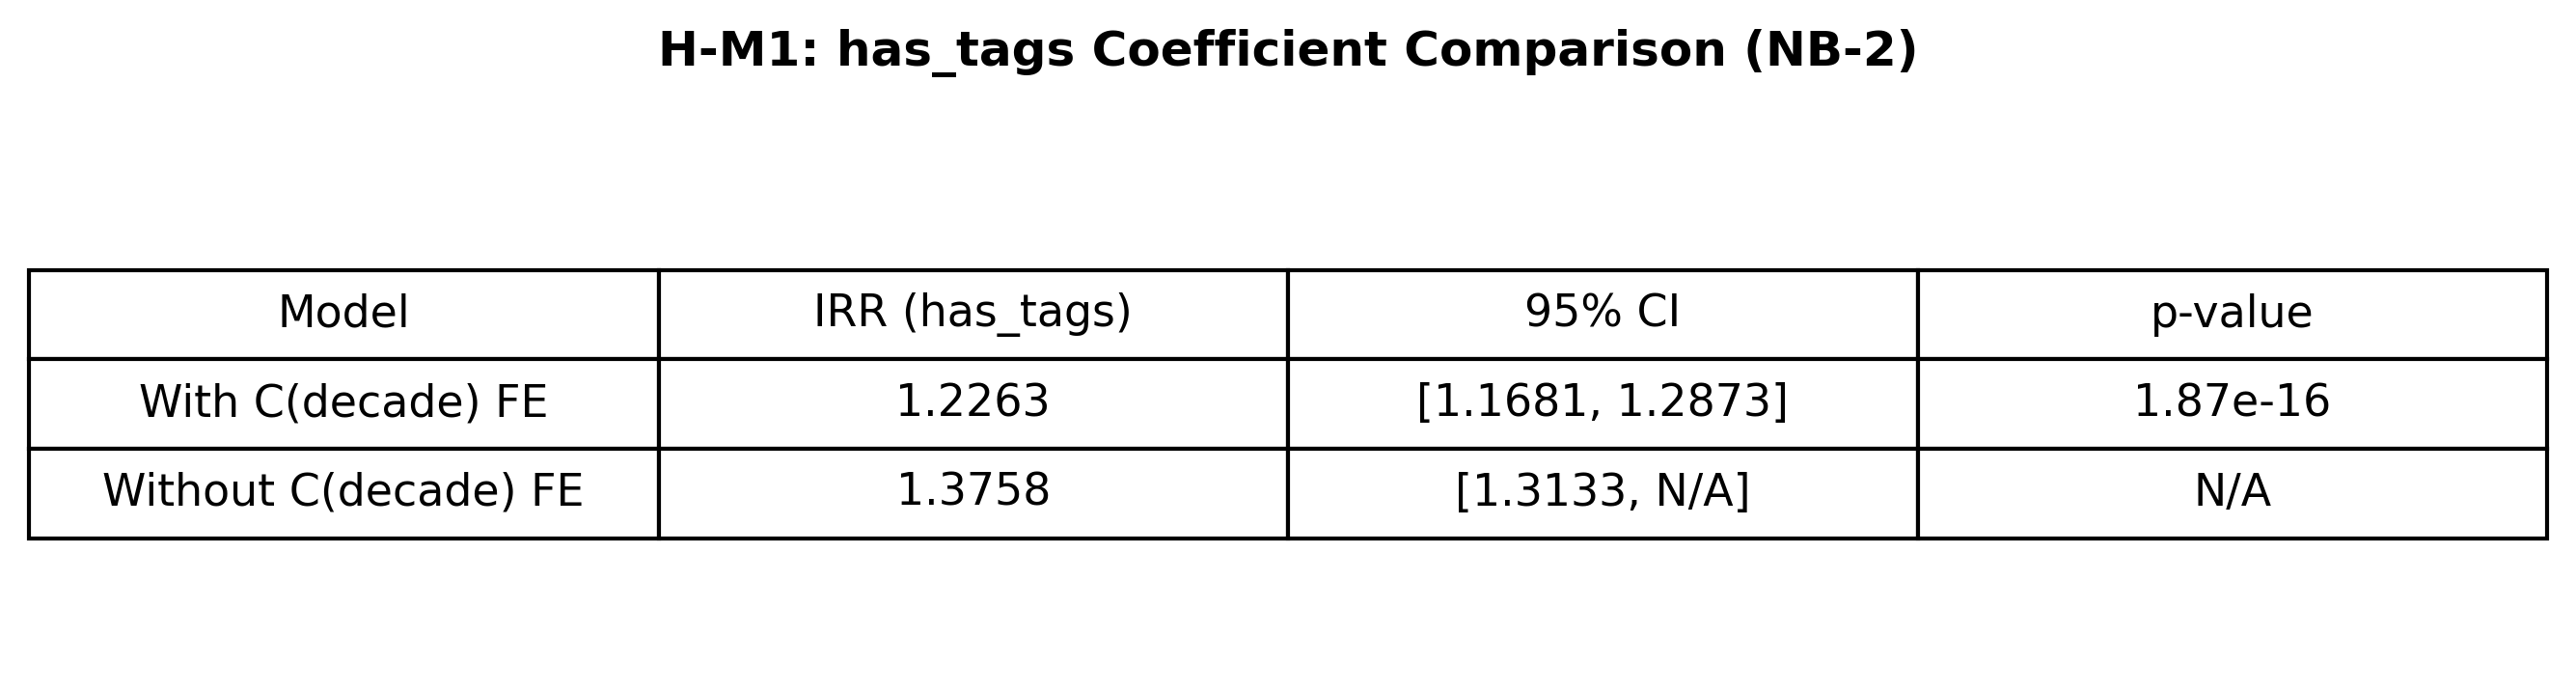
\includegraphics[width=0.65\linewidth]{figures/fig3_coefficient_table.png}
\caption{Full NB-2 coefficient table for the primary model (P1). All covariates and decade fixed effects shown.}
\label{fig:coef_table}
\end{figure}

\begin{figure}[h]
\centering
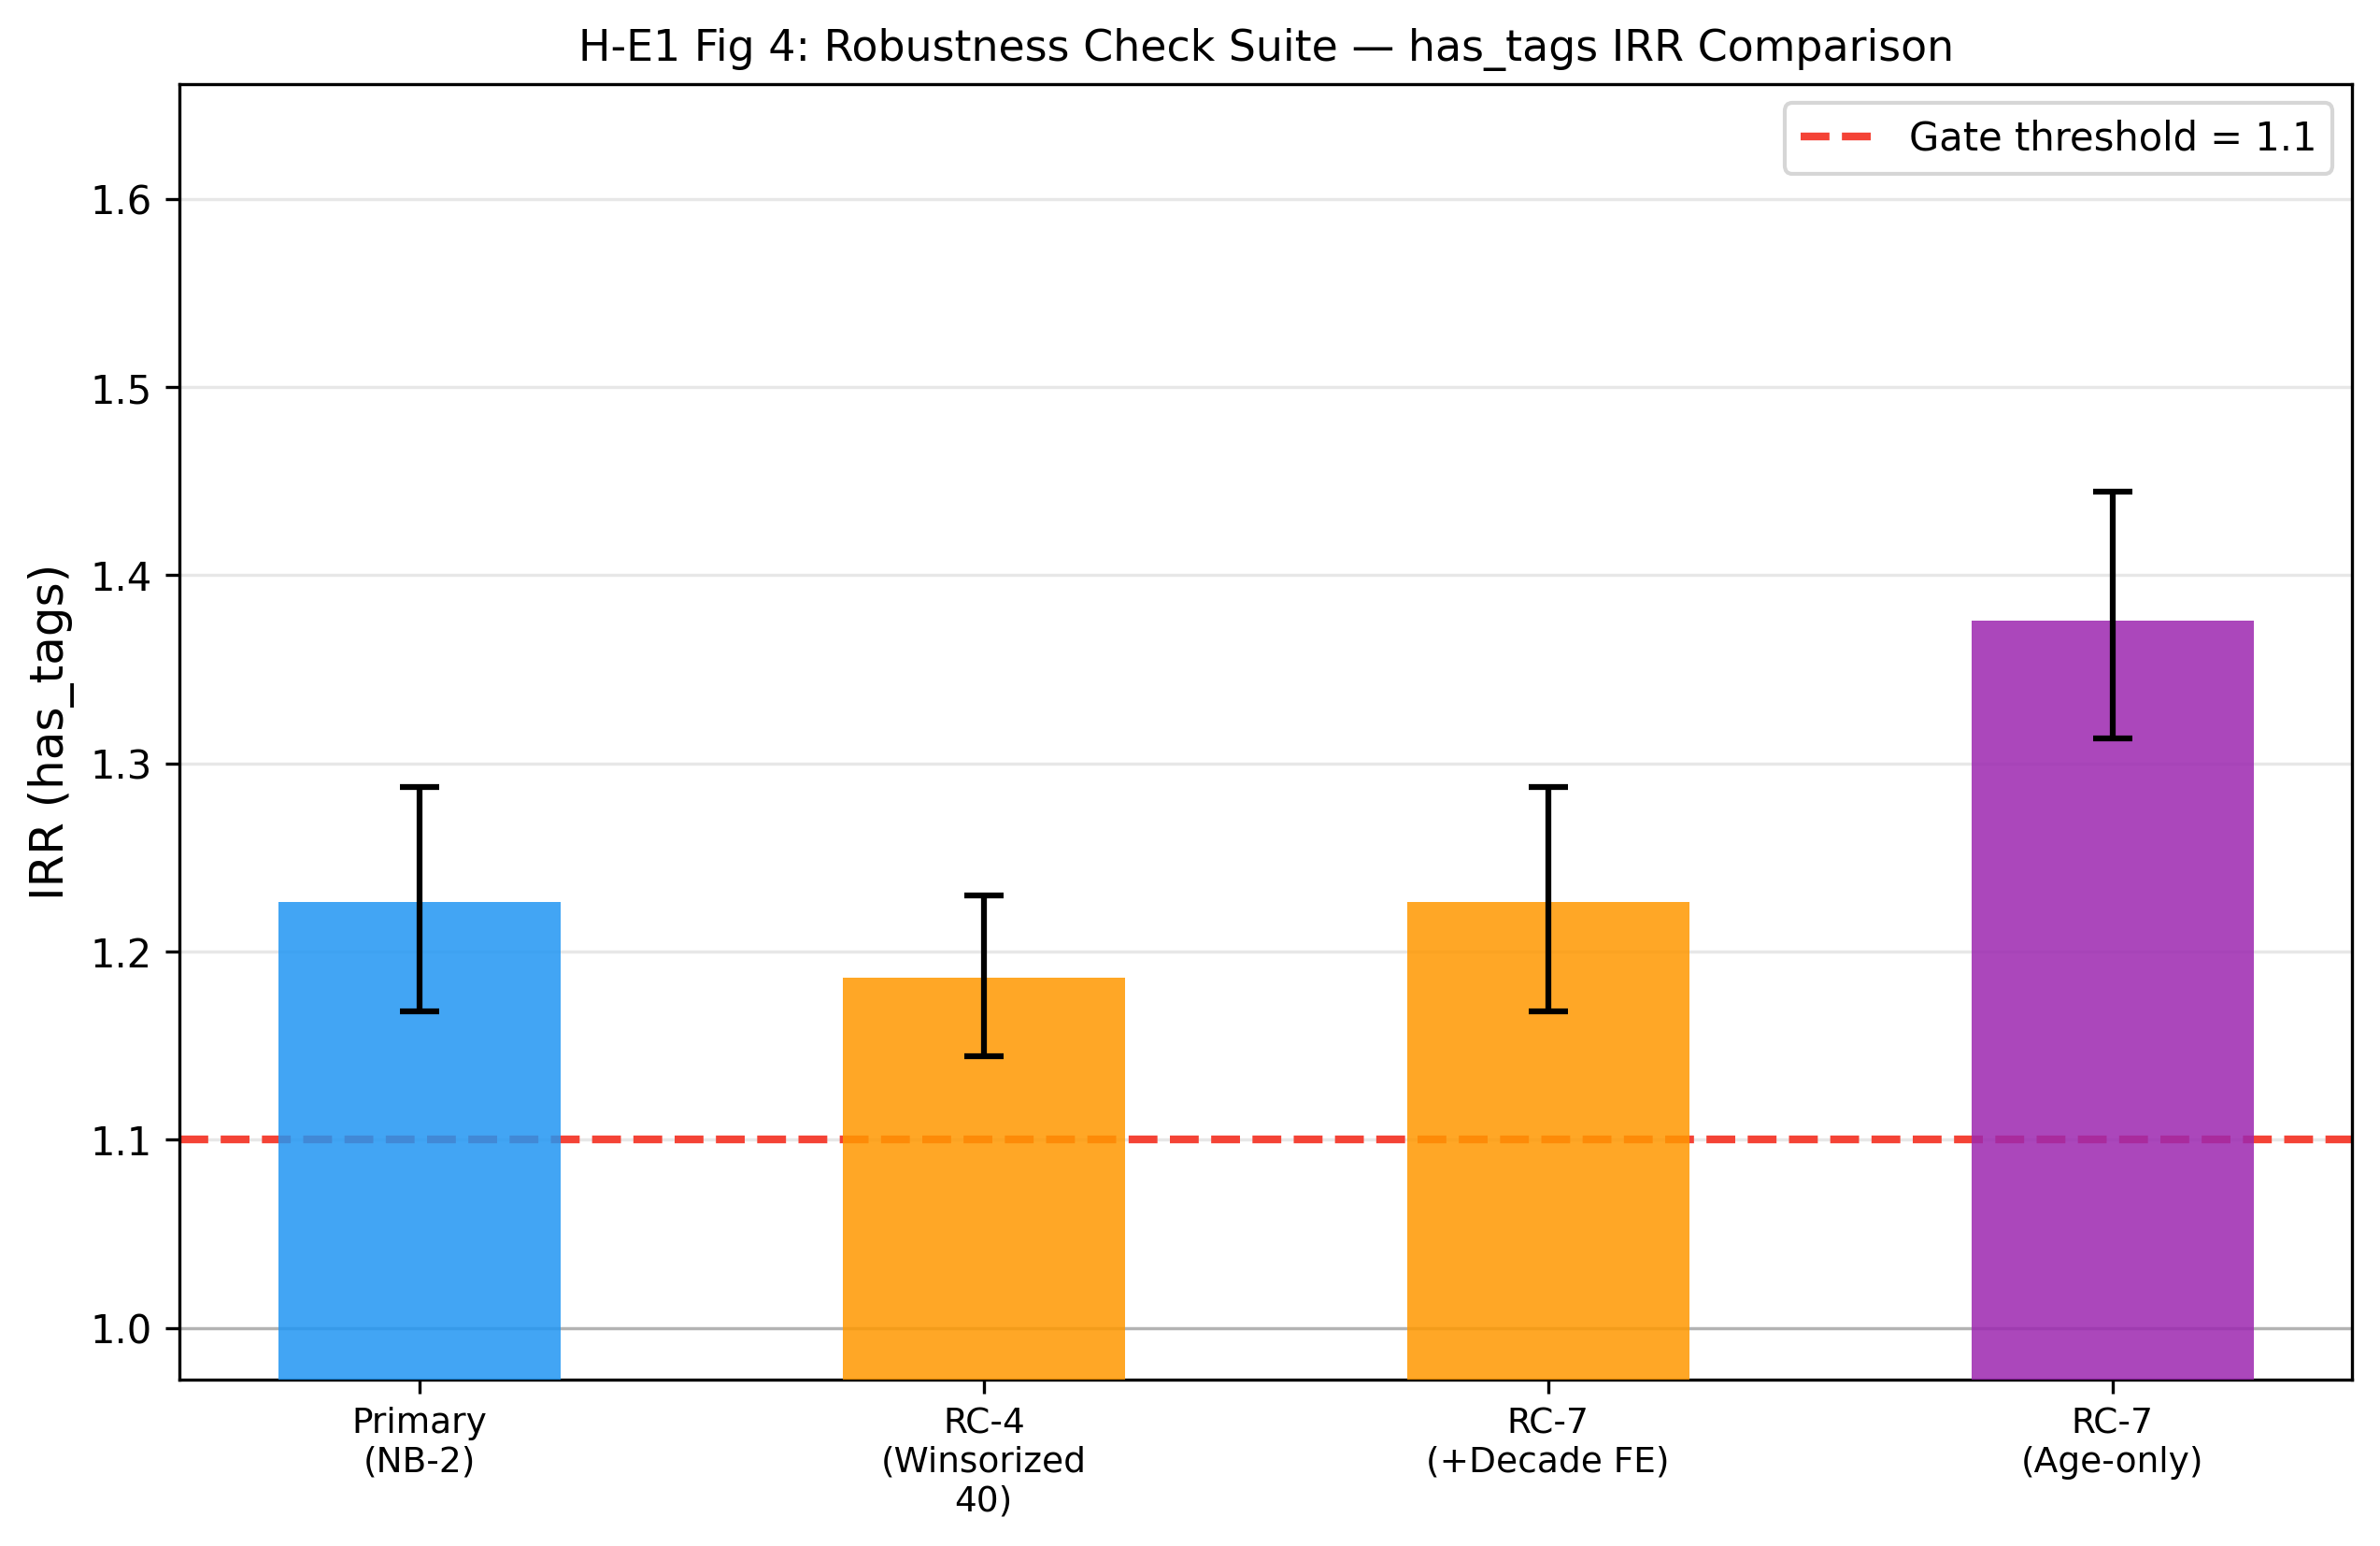
\includegraphics[width=0.65\linewidth]{figures/fig4_rc_comparison.png}
\caption{Robustness check comparison: IRR estimates for \texttt{has\_tags} under RC-4 (winsorization) and RC-7 (age-only FE). Gate passes in all variants.}
\label{fig:rc_comparison}
\end{figure}

\begin{figure}[h]
\centering
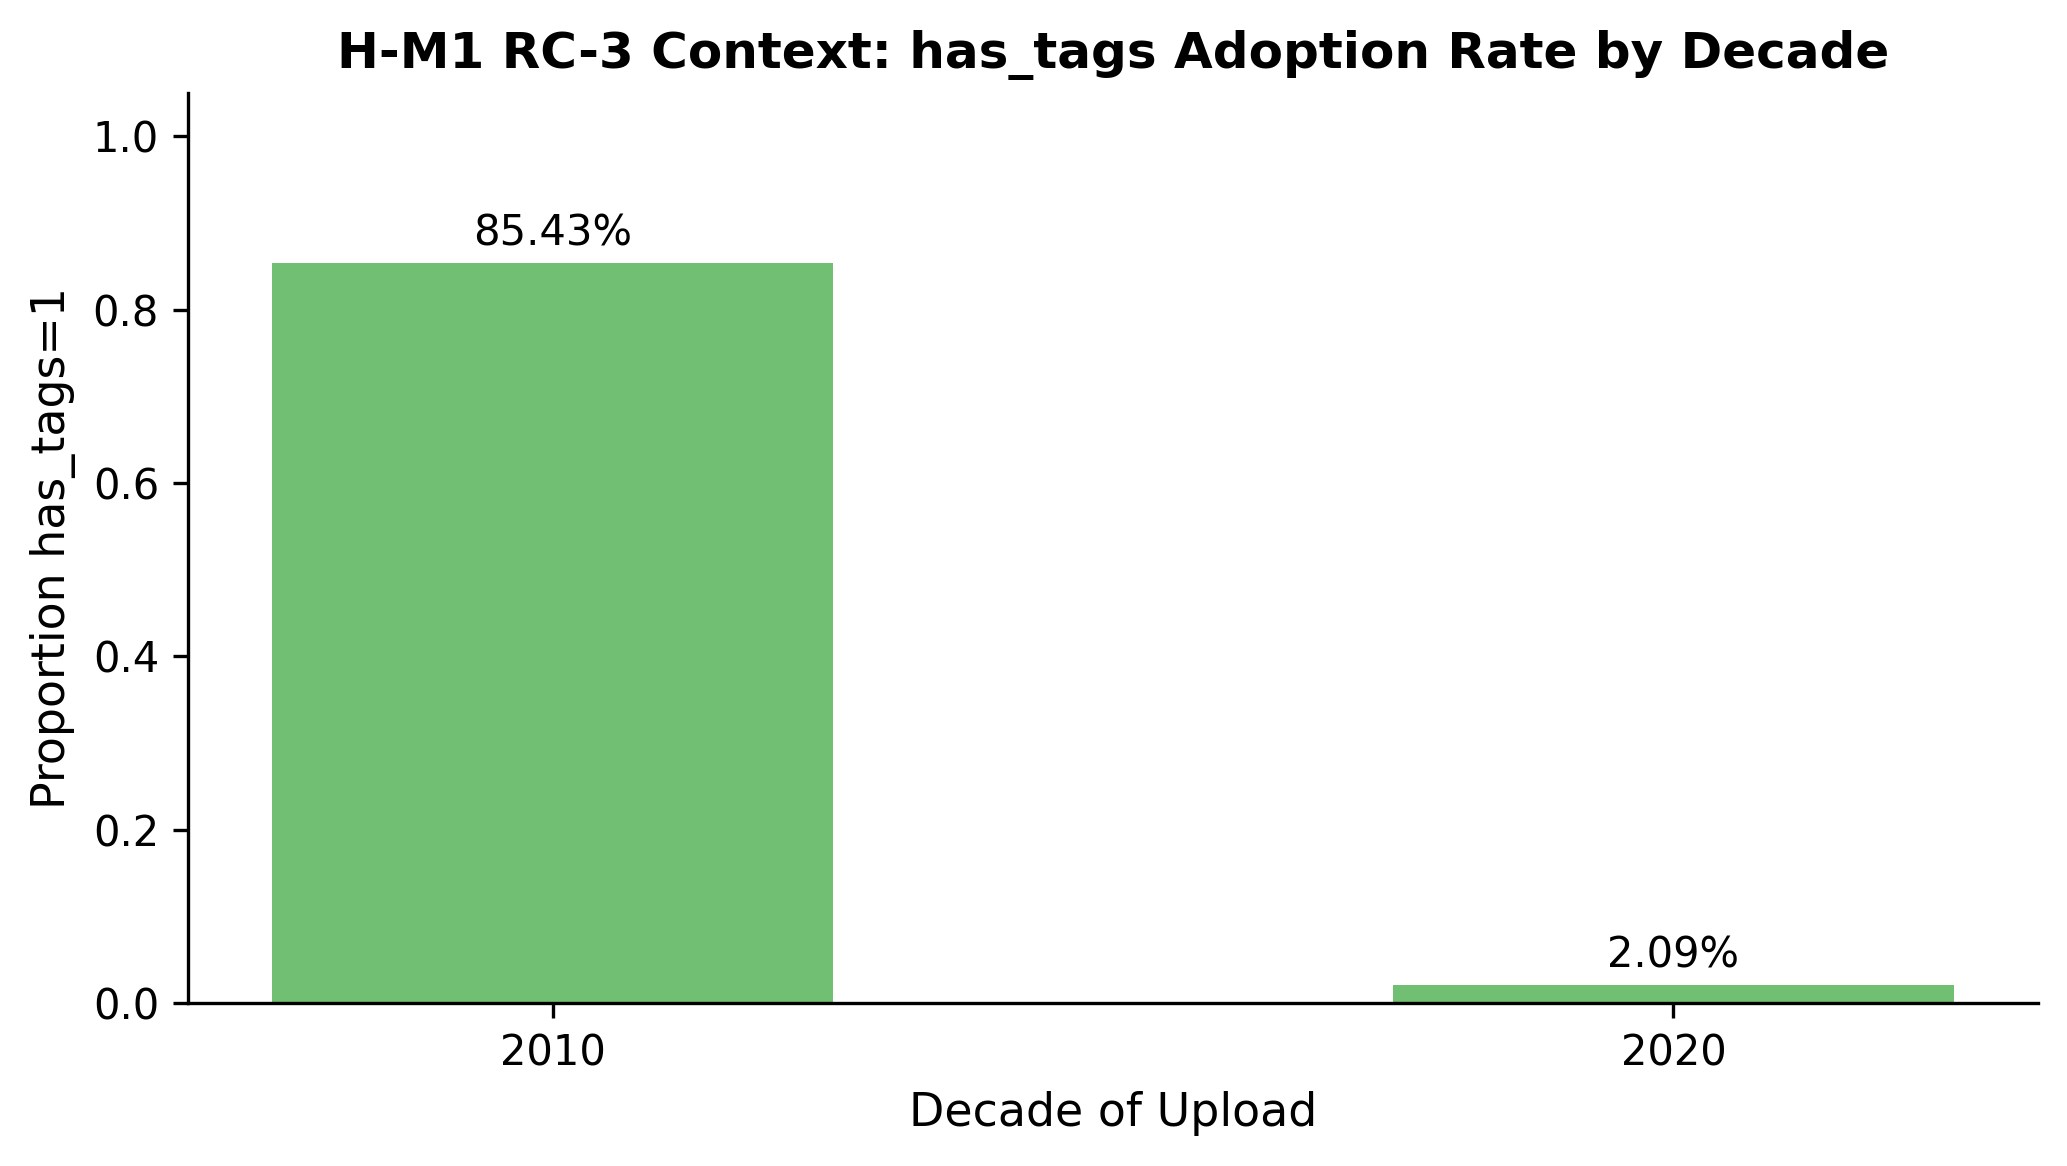
\includegraphics[width=0.65\linewidth]{figures/fig2_hastags_by_decade.png}
\caption{Proportion of tagged datasets by upload decade. Tag adoption increased sharply from 2000s to 2010s, creating the collinearity challenge addressed by decade FE.}
\label{fig:tags_by_decade}
\end{figure}


\end{document}
